\chapter{Case Study: Prediction of Dynamical Properties of Biochemical Pathways using Deep Graph Networks}\label{ch:prediction-biochemical-dgn}

In this chapter, we present an application of Deep Learning techniques on graphs to a life sciences problem related to computational biology. Specifically, we apply Deep Graph Networks to process biochemical pathways, \ie dynamical systems that model the complex interactions between molecules at the biochemical level. Biochemical pathways can be represented as a particular form of bipartite graphs known as Petri networks, which allow to study several properties of such systems. Here, we focus on the property of concentration robustness. To be measured, concentration robustness requires to perform time-expensive simulations. Here, we opt for an approximate but reliable solution, which is orders of magnitude faster to compute. Through processing of the Petri network associated to the biochemical pathway with Deep Graph Networks, we show experimentally that it is possible to build a model that predicts concentration robustness rapidly and with a satisfactory level of accuracy.

\section{Introduction and Motivation}
In order to understand the mechanisms underlying the functioning of living cells, it is necessary to analyze their activities at the biochemical level. Biochemical pathways (or pathways, in short) are complex dynamical systems in which molecules interact with each other through chemical reactions. In these reactions, molecules can take the role of reactant, product, promoter or inhibitor. The dynamics of a pathway are determined by the variation over time of the concentration of its molecules. To study these dynamics, two methodologies are traditionally employed. One consists in modelling the pathway as a system of \glspl{ode}, derived from the application of chemical kinetics laws such as the law of mass action. In cases where pathways involve molecules available in small concentrations, which make the dynamics of reactions sensitive to random events, stochastic modelling and simulation approaches are preferred. These are usually variants of the well-known Gillespie's simulation algorithm \citep{gillespie1977exact}. The use of these modelling tools allows to investigate dynamical properties of biochemical pathways such as the reachability of steady states, the occurrence of oscillatory behaviors, causalities between molecular species, and robustness. However, quantitatively measuring these properties often requires to execute a large number of numerical or stochastic simulation, which in turn are time-consuming and computationally intensive.

Given their nature, one widely used formalism to represent biochemical pathways is that of graphs. Many different graphical notations of pathways exist in the literature (see, e.g., \citet{karp1994representations,reddy1993petri,le2009systems}), most of which represent molecules as nodes, and reactions as multi-edges or as additional nodes. Using graphs to represent pathways is convenient for three main reasons. Firstly, they provide a quite natural visual representation of the reactions occurring in the pathway. Secondly, they enable the study of the pathway dynamics through methods such as network and structural analysis. Thirdly, graphs can easily be transformed into \glspl{ode} or stochastic models, to apply standard numerical simulation techniques.

In this study, we investigate whether predicting dynamical properties of biochemical pathways from the structure of their associated graphs is possible; and if so, to what extent. In other words, our main assumption is that the dynamics of the biological system modeled by the pathway can be correlated to the structural properties of the graph by which it is represented. If the assumption is correct, the positive implications are two-fold: on one hand, a good predictive model of desired biochemical properties could, in principle, replace numerical or stochastic simulations whenever time and computational budgets are limited. On the other hand, it could allow to predict the properties even in cases where the quantitative information is not available, for example whenever numerical or stochastic simulation methods cannot be applied.

The main idea behind this work is to use of Deep Graph Networks to learn structural features of pathways represented as Petri networks (or Petri nets, in short), which are used to predict a property of interest. Here, we focus on the assessment of the dynamical property of robustness, defined as the the ability of a pathway to preserve its dynamics despite the perturbation of some parameters or initial conditions. More specifically, given a pathway and a pair of molecular species (called \emph{input} and \emph{output} species), the robustness measures how much the concentration of the output species at the steady state is influenced by perturbations of the initial concentration of the input species. This is a notion of \emph{concentration robustness} \citep{kitano2004biological} which is to some extent correlated with the notion of global sensitivity \citep{zi2011sensitivity}. Robustness makes up for a perfect candidate to test our approach, as its assessment is time-consuming and computationally intensive, requiring a huge number of simulations to explore the parameters space.

The initial part of this work focuses on the creation of a dataset suited to train the \gls{dgn}. We start from collecting 706 curated pathway models in SBML format from the BioModels\footnote{BioModels: \url{https://www.ebi.ac.uk/biomodels/}} database \citep{li2010biomodels}, which were initially converted into Petri nets. For every pathway in this initial dataset, the robustness of every possible pair of input and output species has been computed through \gls{ode}-based simulations. Then, these robustness values have been transformed into binary indicators of whether robustness holds for a given pathway and input/output species. Lastly, for each pathway and for each input/output species in that pathway, the induced subgraphs containing the input and output nodes (as well as other nodes that influence the pathway dynamics) have been extracted. To summarize, the final dataset obtained with this preparatory phase consists of a set of subgraphs, each associated to a pair of input/output molecular species, and their respective robustness indicator. The predictive task is thus one of binary classification: specifically, given a subgraph and two nodes corresponding to the input and output species, the model should correctly classify them as robust or not.

We model the task with a \gls{dgn} to learn structural features from the subgraphs and compute a graph embedding that is passed to a \gls{mlp} classifier. The performances of the model are assessed according to a rigorous framework similar to the one developed in \ref{sec:comparison-exp-setup}. Our experimental results show that we are indeed able to predict robustness with reasonable accuracy. We also conduct a follow-up investigation of how the architectural choices, such as type of graph convolutional layer and number of layer, impact performances. The analysis suggests that the depth of the \gls{dgn}, in terms of number of layers, plays an important role in capturing the right features that correlate the subgraph structure to the robustness, and that deep \glspl{dgn} perform better at this task.

To our knowledge, this is the first work that addresses the problem of predicting dynamical, properties of pathways on a large scale using Deep Learning. In contrast, other approaches in the literature mainly focus on inferring the parameters of a single pathway, or the relationships between its species. We believe this work has great potential in helping understand the functioning of living cells, by serving as a fast, and computationally friendlier, alternative to performing expensive simulations in the assessment of pathway properties.

\section{Background}\label{sect:background}
In this section, we provide the necessary formal background to understand the modeling of biochemical pathways with Petri nets, and the dynamical property of concentration robustness.

\subsection{Pathway Petri Nets}\label{sec:ppn}
Biochemical pathways are essentially sets of chemical reactions of the form:
\[
c_1 S_1 + c_2 S_2 + \ldots
\xrightarrow{k}
c_1' P_1 + c_2' P_2 \ldots,
\]
where $S_i,P_i$ are molecules (\emph{reactants} and \emph{products}, respectively), $c_i, c_i' \in \Natural$ are \emph{stoichiometric coefficients} expressing the multiplicities of reactants and products involved in the reaction, and $k \in \Real_{\geq 0}$ is the \emph{kinetic constant}, used to compute the reaction rate according to standard chemical kinetic laws such as the law of mass action. Besides reactants and products, the reactions of a biochemical pathway often include in their description other molecules, called \emph{modifiers}. These are not consumed nor produced by the reaction, but act either as \emph{promoters} or as \emph{inhibitors}, meaning that they can increase or decrease the reaction rate, respectively. Although these molecules are not listed among reactants and products, they do have a role in the kinetic formula, which no longer follows the mass action principle in this case. For example, in the SBML language \citep{hucka2018sbml}, a standard XML-based modeling language for biochemical pathways, reactions can be associated with a number of modifiers, whose concentration is used in the kinetic formula of the reaction. In Figure \ref{subfig:example-reactions} we show a table describing the set of reactions describing a biochemical pathway (first column), some of which include a modifier (second column), namely $A$ for the third reaction, and $F$ for the sixth. Each reaction is associated with its kinetic formula (third column), that, for simplicity, we reference through an alias of the form $\mathsf{r}i$ with $i = 1, \ldots, 7$. Using the kinetic formulas of the two reactions with modifiers as an example, it is clear that $A$ acts as a promoter (meaning that the reaction rate is proportional to the concentration of $A$) and that $F$ acts as inhibitor (meaning that the reaction rate is inversely proportional to the concentration of $F$). Kinetic formulas can then be used to construct a system of \glspl{ode} as shown in Figure \ref{subfig:example-odes}.

\begin{figure}
\begin{subfigure}[b]{0.49\linewidth}
    \[\def\arraystretch{1.2}
    \begin{array}{ccl}
      \mbox{Reaction } & \mbox{ Modifiers } & \mbox{ Kinetics}\\
      \hline
      \SF{A} + \SF{B} \rightarrow 2\SF{B} &      & \SF{r}1 = k_1\SF{AB}\\
      \SF{B} \rightarrow \SF{A}      &      & \SF{r}2 = k_2\SF{B}\\
      \SF{C} + \SF{D} \rightarrow \SF{E}  & \SF{A}    & \SF{r}3 = k_3\SF{CDA}\\
      \SF{E} \rightarrow \SF{F}      &      & \SF{r}4 = k_4\SF{E}\\
      \SF{F} \rightarrow \SF{E}      &      & \SF{r}5 = k_5\SF{F}\\
      \SF{G} \rightarrow \SF{H}      & \SF{F}    & \SF{r}6 = \frac{k_6\SF{G}}{1+2 \SF{F}}\\
      \SF{H} \rightarrow \SF{G}      &      & \SF{r}7 = k_7\SF{H}\\
    \end{array}
    \]
\caption{Reactions}\label{subfig:example-reactions}
\end{subfigure}
%
\begin{subfigure}[b]{0.49\linewidth}
\[\def\arraystretch{1.2}
\begin{array}{l}
    \frac{d\SF{A}}{dt} = -k_1\SF{A}B + k_2\SF{B}\\
    \frac{d\SF{B}}{dt} = k_1\SF{AB} - k_2\SF{B}\\
    \frac{d\SF{C}}{dt} = -k_3\SF{CDA}\\
    \frac{d\SF{D}}{dt} = -k_3\SF{CDA}\\
    \frac{d\SF{E}}{dt} = k_3\SF{CDA} - k_4\SF{E} + k_5\SF{F}\\
    \frac{d\SF{F}}{dt} = k_4\SF{E} - k_5\SF{F}\\
    \frac{d\SF{G}}{dt} = -\frac{k_6\SF{G}}{1+2 \SF{F}} + k_7\SF{H}\\
    \frac{d\SF{H}}{dt} = \frac{k_6\SF{G}}{1+2 \SF{F}} - k_7\SF{H}
\end{array}
\]
\caption{ODEs}\label{subfig:example-odes}
\end{subfigure}
%
\caption{An example of biochemical pathway. ({\scriptsize A}) list of reactions with information on modifiers and kinetic formulas. ({\scriptsize B}) the corresponding system of ODEs.}\label{fig:example-pathway}
\end{figure}

A common way to represent biochemical pathways is through Petri nets. The formalism of Petri nets have been originally proposed for the description and analysis of concurrent systems \citep{peterson1977petri}, but has been later adopted to model other kinds of systems, such as biological ones. Several variants of Petri nets have been proposed in the literature. In this work, we consider a version of \emph{continuous} Petri nets \citep{gilbert2007petri} with promotion and inhibition edges and general kinetic functions. We call this biologically inspired variant \gls{ppn}. A \gls{ppn} is essentially a bipartite graph with two types of nodes and three types of labelled edges. According to standard Petri nets terminology, the two types of nodes are called \emph{places} and \emph{transitions}. The semantics of a \gls{ppn} in a continuous setting are described by a system of ODEs, with one equation for each place. In the case of pathways, such system corresponds exactly to the one obtained from the chemical reactions shown in Figure \ref{subfig:example-odes}. The state of a \gls{ppn} (called \emph{marking}) is then defined as an assignment of positive real values to the variables of the ODEs. We denote with $\Cal{M}$ the set of all possible markings.

More formally, a \gls{ppn} can be defined as a tuple $\wp = \Tuple{\Cal{P},\Cal{T},\Cal{A}_{S}, \Cal{A}_{P},\Cal{A}_{I},\vartheta,\varsigma,M_0}$ where:
\begin{itemize}
    \item $\Cal{P}$ and $\Cal{T}$ are finite, non empty disjoint sets of places and transitions, respectively;
    \item $\Cal{A}_{S} = ((\Cal{P}\times \Cal{T}) \cup (\Cal{T}\times \Cal{P})$ is a set of standard directed edges;
    \item $\Cal{A}_{P} \subseteq (\Cal{P} \times \Cal{T})$ is the set of promotion edges;
    \item $\Cal{A}_{I} \subseteq (\Cal{P} \times \Cal{T})$ is the set of inhibition edges;
    \item $\varsigma: \Cal{A}_{S} \shortrightarrow \mathbb{N}^{\geq 0}$ weights every standard edge by non-negative integer values;
    \item $\varsigma:\Cal{T} \shortrightarrow (\Cal{M} \rightarrow \mathbb{R}^{\geq 0})$,  is a function that assigns, to each transition, a function that computes a kinetic formula to every possible marking $M \in \Cal{M}$;
    \item $M_0 \in \Cal{M}$ is the initial marking.
\end{itemize}
A visual representation of the \gls{ppn} corresponding to the pathway in Figure \ref{subfig:example-reactions} is shown in Figure \ref{subfig:pathway-petri-net}. The sets of places $\Cal{P}$ and transitions $\Cal{T}$ of a pathway Petri net represent molecular species and reactants, and are displayed as circles and rectangles, respectively. In the figure, places are labeled with the name of the corresponding molecule. The directed edges, depicted as standard arrows, connect reactants to reactions and reactions to products. The weights of the edges (omitted if equal to one) correspond to the stoichiometric coefficients of reactant/product pairs. The sets of promotion and inhibition edges, $\Cal{A}_{P}$ and $\Cal{A}_{I}$, connect molecules to the reactions they promote or inhibit, respectively, and they are displayed as dotted or T-shaped arrows, respectively. The kinetic formulas of reactions (or rather, their aliases defined as in Figure \ref{subfig:pathway-petri-net}), are shown inside the rectangles of the corresponding transitions. As explained previously, molecules connected through promotion edges give a positive contribution to the value of the kinetic formula, while molecules connected through inhibition edges give a negative (inversely proportional) contribution. Finally, the initial marking $M_0$ is not shown in the figure, and it has to be described separately.
\begin{figure*}[h!]
    \centering
    \resizebox{.6\textwidth}{!}{

\tikzset{every picture/.style={line width=0.75pt}} %set default line width to 0.75pt        

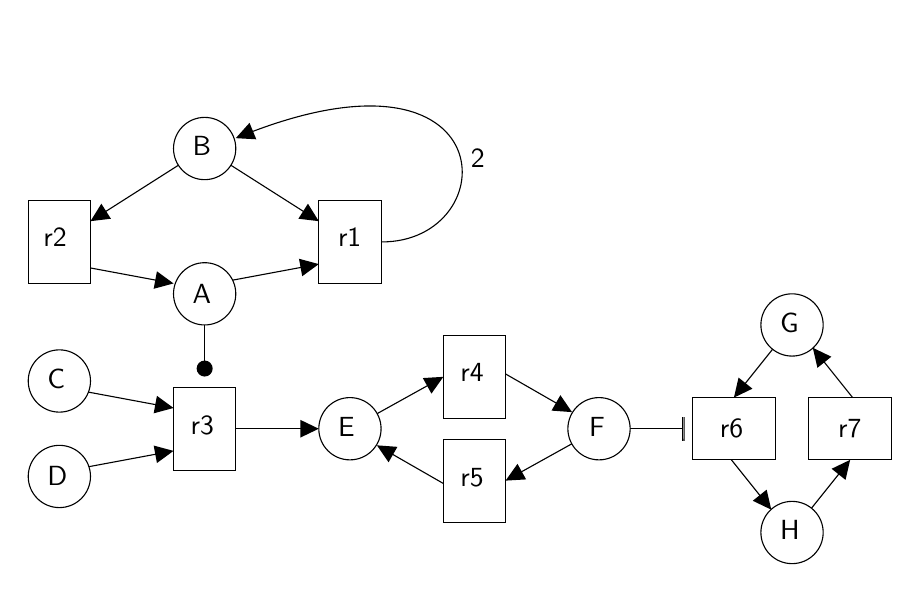
\begin{tikzpicture}[x=0.75pt,y=0.75pt,yscale=-1,xscale=1]
%uncomment if require: \path (0,300); %set diagram left start at 0, and has height of 300

%Straight Lines [id:da3576438741903769] 
\draw    (388,210) -- (414.13,177.34) ;
\draw [shift={(416,175)}, rotate = 488.66] [fill={rgb, 255:red, 0; green, 0; blue, 0 }  ][line width=0.08]  [draw opacity=0] (8.93,-4.29) -- (0,0) -- (8.93,4.29) -- cycle    ;
%Straight Lines [id:da5206527388854192] 
\draw    (350,164) -- (376.13,196.66) ;
\draw [shift={(378,199)}, rotate = 231.34] [fill={rgb, 255:red, 0; green, 0; blue, 0 }  ][line width=0.08]  [draw opacity=0] (8.93,-4.29) -- (0,0) -- (8.93,4.29) -- cycle    ;
%Straight Lines [id:da9664135693242828] 
\draw    (388,110) -- (361.87,142.66) ;
\draw [shift={(360,145)}, rotate = 308.65999999999997] [fill={rgb, 255:red, 0; green, 0; blue, 0 }  ][line width=0.08]  [draw opacity=0] (8.93,-4.29) -- (0,0) -- (8.93,4.29) -- cycle    ;
%Straight Lines [id:da3150124855239005] 
\draw    (426,156) -- (399.87,123.34) ;
\draw [shift={(398,121)}, rotate = 411.34000000000003] [fill={rgb, 255:red, 0; green, 0; blue, 0 }  ][line width=0.08]  [draw opacity=0] (8.93,-4.29) -- (0,0) -- (8.93,4.29) -- cycle    ;
%Straight Lines [id:da2531638133399581] 
\draw    (295,160) -- (335,160) ;
%Straight Lines [id:da7978054588524539] 
\draw    (110,160) -- (157,160) ;
\draw [shift={(160,160)}, rotate = 180] [fill={rgb, 255:red, 0; green, 0; blue, 0 }  ][line width=0.08]  [draw opacity=0] (8.93,-4.29) -- (0,0) -- (8.93,4.29) -- cycle    ;
%Straight Lines [id:da5621074466789615] 
\draw    (235,125) -- (279.4,150.51) ;
\draw [shift={(282,152)}, rotate = 209.88] [fill={rgb, 255:red, 0; green, 0; blue, 0 }  ][line width=0.08]  [draw opacity=0] (8.93,-4.29) -- (0,0) -- (8.93,4.29) -- cycle    ;
%Straight Lines [id:da9432384230142636] 
\draw    (235,195) -- (190.6,169.49) ;
\draw [shift={(188,168)}, rotate = 389.88] [fill={rgb, 255:red, 0; green, 0; blue, 0 }  ][line width=0.08]  [draw opacity=0] (8.93,-4.29) -- (0,0) -- (8.93,4.29) -- cycle    ;
%Straight Lines [id:da2732887752012232] 
\draw    (295,160) -- (252.62,183.54) ;
\draw [shift={(250,185)}, rotate = 330.95] [fill={rgb, 255:red, 0; green, 0; blue, 0 }  ][line width=0.08]  [draw opacity=0] (8.93,-4.29) -- (0,0) -- (8.93,4.29) -- cycle    ;
%Straight Lines [id:da8361705783456022] 
\draw    (175,160) -- (217.38,136.46) ;
\draw [shift={(220,135)}, rotate = 510.95] [fill={rgb, 255:red, 0; green, 0; blue, 0 }  ][line width=0.08]  [draw opacity=0] (8.93,-4.29) -- (0,0) -- (8.93,4.29) -- cycle    ;
%Straight Lines [id:da26704871020062715] 
\draw    (110,90) -- (157.05,81.23) ;
\draw [shift={(160,80.68)}, rotate = 529.44] [fill={rgb, 255:red, 0; green, 0; blue, 0 }  ][line width=0.08]  [draw opacity=0] (8.93,-4.29) -- (0,0) -- (8.93,4.29) -- cycle    ;
%Straight Lines [id:da4846937260313433] 
\draw    (40,80.68) -- (87.05,89.45) ;
\draw [shift={(90,90)}, rotate = 190.56] [fill={rgb, 255:red, 0; green, 0; blue, 0 }  ][line width=0.08]  [draw opacity=0] (8.93,-4.29) -- (0,0) -- (8.93,4.29) -- cycle    ;
%Straight Lines [id:da271105016276878] 
\draw    (105,25) -- (157.47,58.39) ;
\draw [shift={(160,60)}, rotate = 212.47] [fill={rgb, 255:red, 0; green, 0; blue, 0 }  ][line width=0.08]  [draw opacity=0] (8.93,-4.29) -- (0,0) -- (8.93,4.29) -- cycle    ;
%Shape: Rectangle [id:dp9228181661849988] 
\draw  [fill={rgb, 255:red, 255; green, 255; blue, 255 }  ,fill opacity=1 ] (20,50) -- (50,50) -- (50,90) -- (20,90) -- cycle ;
%Straight Lines [id:da06467494297119436] 
\draw    (105,25) -- (52.53,58.39) ;
\draw [shift={(50,60)}, rotate = 327.53] [fill={rgb, 255:red, 0; green, 0; blue, 0 }  ][line width=0.08]  [draw opacity=0] (8.93,-4.29) -- (0,0) -- (8.93,4.29) -- cycle    ;
%Shape: Circle [id:dp49236484975772] 
\draw  [fill={rgb, 255:red, 255; green, 255; blue, 255 }  ,fill opacity=1 ] (90,25) .. controls (90,16.72) and (96.72,10) .. (105,10) .. controls (113.28,10) and (120,16.72) .. (120,25) .. controls (120,33.28) and (113.28,40) .. (105,40) .. controls (96.72,40) and (90,33.28) .. (90,25) -- cycle ;
%Shape: Rectangle [id:dp3146550401206405] 
\draw  [fill={rgb, 255:red, 255; green, 255; blue, 255 }  ,fill opacity=1 ] (160,50) -- (190,50) -- (190,90) -- (160,90) -- cycle ;
%Curve Lines [id:da9984566963389516] 
\draw    (190,70) .. controls (250.06,70.4) and (250.75,-32.96) .. (121.95,19.2) ;
\draw [shift={(120,20)}, rotate = 337.56] [fill={rgb, 255:red, 0; green, 0; blue, 0 }  ][line width=0.08]  [draw opacity=0] (8.93,-4.29) -- (0,0) -- (8.93,4.29) -- cycle    ;
%Shape: Circle [id:dp09345090103745823] 
\draw  [fill={rgb, 255:red, 255; green, 255; blue, 255 }  ,fill opacity=1 ] (90,95) .. controls (90,86.72) and (96.72,80) .. (105,80) .. controls (113.28,80) and (120,86.72) .. (120,95) .. controls (120,103.28) and (113.28,110) .. (105,110) .. controls (96.72,110) and (90,103.28) .. (90,95) -- cycle ;
%Straight Lines [id:da5223576478149881] 
\draw    (105,110) -- (105,131) ;
\draw [shift={(105,131)}, rotate = 90] [color={rgb, 255:red, 0; green, 0; blue, 0 }  ][fill={rgb, 255:red, 0; green, 0; blue, 0 }  ][line width=0.75]      (0, 0) circle [x radius= 3.35, y radius= 3.35]   ;
%Shape: Rectangle [id:dp25364205729175127] 
\draw  [fill={rgb, 255:red, 255; green, 255; blue, 255 }  ,fill opacity=1 ] (90,140) -- (120,140) -- (120,180) -- (90,180) -- cycle ;
%Straight Lines [id:da8084682726089965] 
\draw    (40,140.68) -- (87.05,149.45) ;
\draw [shift={(90,150)}, rotate = 190.56] [fill={rgb, 255:red, 0; green, 0; blue, 0 }  ][line width=0.08]  [draw opacity=0] (8.93,-4.29) -- (0,0) -- (8.93,4.29) -- cycle    ;
%Straight Lines [id:da8278541197200837] 
\draw    (40,180) -- (87.05,171.23) ;
\draw [shift={(90,170.68)}, rotate = 529.44] [fill={rgb, 255:red, 0; green, 0; blue, 0 }  ][line width=0.08]  [draw opacity=0] (8.93,-4.29) -- (0,0) -- (8.93,4.29) -- cycle    ;
%Shape: Circle [id:dp5697702501712039] 
\draw  [fill={rgb, 255:red, 255; green, 255; blue, 255 }  ,fill opacity=1 ] (20,137) .. controls (20,128.72) and (26.72,122) .. (35,122) .. controls (43.28,122) and (50,128.72) .. (50,137) .. controls (50,145.28) and (43.28,152) .. (35,152) .. controls (26.72,152) and (20,145.28) .. (20,137) -- cycle ;
%Shape: Circle [id:dp027027959729662543] 
\draw  [fill={rgb, 255:red, 255; green, 255; blue, 255 }  ,fill opacity=1 ] (20,183) .. controls (20,174.72) and (26.72,168) .. (35,168) .. controls (43.28,168) and (50,174.72) .. (50,183) .. controls (50,191.28) and (43.28,198) .. (35,198) .. controls (26.72,198) and (20,191.28) .. (20,183) -- cycle ;
%Shape: Circle [id:dp7929646959402241] 
\draw  [fill={rgb, 255:red, 255; green, 255; blue, 255 }  ,fill opacity=1 ] (160,160) .. controls (160,151.72) and (166.72,145) .. (175,145) .. controls (183.28,145) and (190,151.72) .. (190,160) .. controls (190,168.28) and (183.28,175) .. (175,175) .. controls (166.72,175) and (160,168.28) .. (160,160) -- cycle ;
%Shape: Rectangle [id:dp05655391624383377] 
\draw  [fill={rgb, 255:red, 255; green, 255; blue, 255 }  ,fill opacity=1 ] (220,115) -- (250,115) -- (250,155) -- (220,155) -- cycle ;
%Shape: Rectangle [id:dp05796590340987029] 
\draw  [fill={rgb, 255:red, 255; green, 255; blue, 255 }  ,fill opacity=1 ] (220,165) -- (250,165) -- (250,205) -- (220,205) -- cycle ;
%Shape: Circle [id:dp13273124949760895] 
\draw  [fill={rgb, 255:red, 255; green, 255; blue, 255 }  ,fill opacity=1 ] (280,160) .. controls (280,151.72) and (286.72,145) .. (295,145) .. controls (303.28,145) and (310,151.72) .. (310,160) .. controls (310,168.28) and (303.28,175) .. (295,175) .. controls (286.72,175) and (280,168.28) .. (280,160) -- cycle ;
%Straight Lines [id:da9347007050049654] 
\draw    (335.29,154.43) -- (335.26,165.81) ;
%Straight Lines [id:da20553639689795267] 
\draw    (336,154.43) -- (335.97,165.81) ;
%Shape: Rectangle [id:dp30165349356224813] 
\draw  [fill={rgb, 255:red, 255; green, 255; blue, 255 }  ,fill opacity=1 ] (380,145) -- (380,175) -- (340,175) -- (340,145) -- cycle ;
%Shape: Rectangle [id:dp05448702121100979] 
\draw  [fill={rgb, 255:red, 255; green, 255; blue, 255 }  ,fill opacity=1 ] (436,145) -- (436,175) -- (396,175) -- (396,145) -- cycle ;
%Shape: Circle [id:dp37659499504730287] 
\draw  [fill={rgb, 255:red, 255; green, 255; blue, 255 }  ,fill opacity=1 ] (373,110) .. controls (373,101.72) and (379.72,95) .. (388,95) .. controls (396.28,95) and (403,101.72) .. (403,110) .. controls (403,118.28) and (396.28,125) .. (388,125) .. controls (379.72,125) and (373,118.28) .. (373,110) -- cycle ;
%Shape: Circle [id:dp13055596917815526] 
\draw  [fill={rgb, 255:red, 255; green, 255; blue, 255 }  ,fill opacity=1 ] (373,210) .. controls (373,201.72) and (379.72,195) .. (388,195) .. controls (396.28,195) and (403,201.72) .. (403,210) .. controls (403,218.28) and (396.28,225) .. (388,225) .. controls (379.72,225) and (373,218.28) .. (373,210) -- cycle ;

% Text Node
\draw (26,62) node [anchor=north west][inner sep=0.75pt]   [align=left] {$\mathsf{r2}$};
% Text Node
\draw (168,62) node [anchor=north west][inner sep=0.75pt]   [align=left] {$\mathsf{r1}$};
% Text Node
\draw (97,153) node [anchor=north west][inner sep=0.75pt]   [align=left] {$\mathsf{r3}$};
% Text Node
\draw (227,127) node [anchor=north west][inner sep=0.75pt]   [align=left] {$\mathsf{r4}$};
% Text Node
\draw (227,178) node [anchor=north west][inner sep=0.75pt]   [align=left] {$\mathsf{r5}$};
% Text Node
\draw (352,154) node [anchor=north west][inner sep=0.75pt]   [align=left] {$\mathsf{r6}$};
% Text Node
\draw (409,154) node [anchor=north west][inner sep=0.75pt]   [align=left] {$\mathsf{r7}$};

% Text Node
\draw (98,18) node [anchor=north west][inner sep=0.75pt]   [align=left] {$\mathsf{B}$};
% Text Node
\draw (98,89) node [anchor=north west][inner sep=0.75pt]   [align=left] {$\mathsf{A}$};
% Text Node
\draw (28,130) node [anchor=north west][inner sep=0.75pt]   [align=left] {$\mathsf{C}$};
% Text Node
\draw (28,177) node [anchor=north west][inner sep=0.75pt]   [align=left] {$\mathsf{D}$};
% Text Node
\draw (168,153) node [anchor=north west][inner sep=0.75pt]   [align=left] {$\mathsf{E}$};
% Text Node
\draw (289,153) node [anchor=north west][inner sep=0.75pt]   [align=left] {$\mathsf{F}$};
% Text Node
\draw (381,103) node [anchor=north west][inner sep=0.75pt]   [align=left] {$\mathsf{G}$};
% Text Node
\draw (381,203) node [anchor=north west][inner sep=0.75pt]   [align=left] {$\mathsf{H}$};
% Text Node
\draw (232,24) node [anchor=north west][inner sep=0.75pt]   [align=left] {$\mathsf{2}$};


\end{tikzpicture}}
    \caption{The Pathway Petri Net corresponding to the reactions described in Figure \ref{subfig:example-reactions}}
    \label{subfig:pathway-petri-net}
\end{figure*}

In this work, we use a variant of \glspl{ppn} where all the information unrelated to the structure of the pathway is discarded. Specifically, we ignore information about:
\begin{itemize}
    \item kinetic formulas;
    \item multiplicities of reactants and products (\ie edge labels);
    \item the initial marking $M_0$.
\end{itemize}
Basically, for our purposes, a \gls{ppn} is a tuple $\wp = \Tuple{\Cal{P},\Cal{T},\Cal{A}_{S}, \Cal{A}_{P},\Cal{A}_{I}}$ where the irrelevant components have been omitted. We rewrite this object, according to the graph notation introduced in Section \ref{sec:graphs}, into a \keyword{pathway graph} $G = \Tuple{\Cal{V}_G, \Cal{E}_G}$. To do so, we first define the following nodes and edges subsets:
\begin{itemize}
    \item $\Cal{V}_{G}^{\Fun{mol}} = \Cal{P}$ is the set of molecules;
    \item $\Cal{V}_{G}^{\Fun{rx}} = \Cal{T}$ is the set of reactions;
    \item $\Cal{E}_{G}^{\Fun{std}} = \Cal{A}_S$ is the set of standard edges;
    \item $\Cal{E}_{G}^{\Fun{pro}} = \Cal{A}_P$ is the set of promoter edges;
    \item $\Cal{E}_{G}^{\Fun{inh}} = \Cal{A}_I$ is the set of inhibitor edges,
\end{itemize}
where $\Cal{V}_{G}^{\Fun{mol}} \Inter \Cal{V}_{G}^{\Fun{rx}} = \emptyset$ and $\Cal{E}_{G}^{\Fun{std}} \Inter \Cal{E}_{G}^{\Fun{pro}} \Inter \Cal{E}_{G}^{\Fun{inh}} = \emptyset$. Then, we simply set $\Cal{V}_G = \Cal{V}_G^{\Fun{mol}} \Union \Cal{V}_G^{\Fun{rx}}$ and $\Cal{E}_G = \Cal{E}_G^{\Fun{std}} \Union \Cal{E}_G^{\Fun{pro}} \Union \Cal{E}_G^{\Fun{inh}}$.
Using the biochemical pathway of Figure \ref{fig:example-pathway} as reference, its associated pathway graph is shown in Figure \ref{fig:pathway-graph}.
\begin{figure*}[h!]
    \centering
    \resizebox{.6\textwidth}{!}{

\tikzset{every picture/.style={line width=0.75pt}} %set default line width to 0.75pt

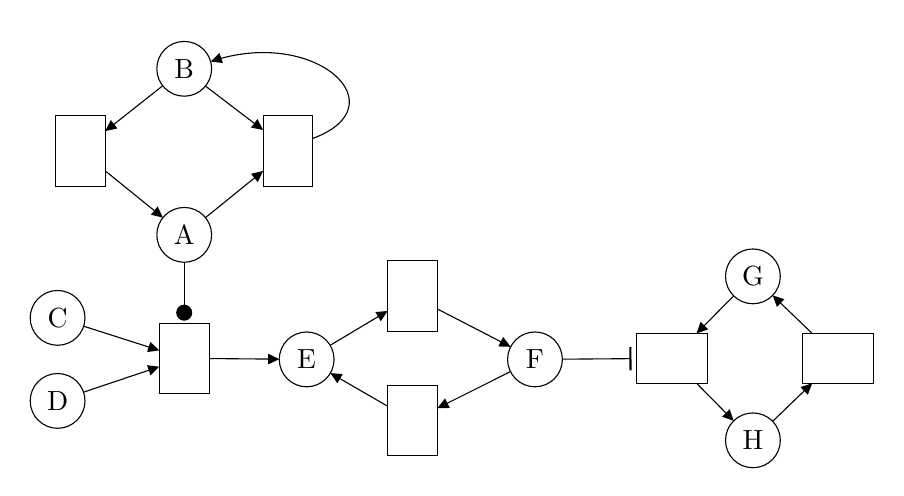
\begin{tikzpicture}[x=0.75pt,y=0.75pt,yscale=-1,xscale=1]
%uncomment if require: \path (0,300); %set diagram left start at 0, and has height of 300

%Straight Lines [id:da289255485986883]
\draw    (100,56) -- (135.62,83.18) ;
\draw [shift={(138,85)}, rotate = 217.35] [fill={rgb, 255:red, 0; green, 0; blue, 0 }  ][line width=0.08]  [draw opacity=0] (5.36,-2.57) -- (0,0) -- (5.36,2.57) -- cycle    ;

% Text Node
\draw  [fill={rgb, 255:red, 255; green, 255; blue, 255 }  ,fill opacity=1 ]  (38,78) -- (62,78) -- (62,112) -- (38,112) -- cycle  ;
\draw (50,95) node   [align=left] {\begin{minipage}[lt]{13.600000000000001pt}\setlength\topsep{0pt}
\begin{center}
\end{center}

\end{minipage}};
% Text Node
\draw  [fill={rgb, 255:red, 255; green, 255; blue, 255 }  ,fill opacity=1 ]  (100, 55.5) circle [x radius= 13.2, y radius= 13.2]   ;
\draw (100,55.5) node   [align=left] {\begin{minipage}[lt]{14.96pt}\setlength\topsep{0pt}
\begin{center}
\SF{B}
\end{center}

\end{minipage}};
% Text Node
\draw  [fill={rgb, 255:red, 255; green, 255; blue, 255 }  ,fill opacity=1 ]  (138,78) -- (162,78) -- (162,112) -- (138,112) -- cycle  ;
\draw (150,95) node   [align=left] {\begin{minipage}[lt]{13.600000000000001pt}\setlength\topsep{0pt}
\begin{center}
\end{center}

\end{minipage}};
% Text Node
\draw  [fill={rgb, 255:red, 255; green, 255; blue, 255 }  ,fill opacity=1 ]  (100, 135.5) circle [x radius= 13.2, y radius= 13.2]   ;
\draw (100,135.5) node   [align=left] {\begin{minipage}[lt]{14.96pt}\setlength\topsep{0pt}
\begin{center}
\SF{A}
\end{center}

\end{minipage}};
% Text Node
\draw  [fill={rgb, 255:red, 255; green, 255; blue, 255 }  ,fill opacity=1 ]  (39, 175.5) circle [x radius= 13.2, y radius= 13.2]   ;
\draw (39,175.5) node   [align=left] {\begin{minipage}[lt]{14.96pt}\setlength\topsep{0pt}
\begin{center}
\SF{C}
\end{center}

\end{minipage}};
% Text Node
\draw  [fill={rgb, 255:red, 255; green, 255; blue, 255 }  ,fill opacity=1 ]  (39, 215.5) circle [x radius= 13.2, y radius= 13.2]   ;
\draw (39,215.5) node   [align=left] {\begin{minipage}[lt]{14.96pt}\setlength\topsep{0pt}
\begin{center}
\SF{D}
\end{center}

\end{minipage}};
% Text Node
\draw  [fill={rgb, 255:red, 255; green, 255; blue, 255 }  ,fill opacity=1 ]  (88,178) -- (112,178) -- (112,212) -- (88,212) -- cycle  ;
\draw (100,195) node   [align=left] {\begin{minipage}[lt]{13.600000000000001pt}\setlength\topsep{0pt}
\begin{center}
\end{center}

\end{minipage}};
% Text Node
\draw  [fill={rgb, 255:red, 255; green, 255; blue, 255 }  ,fill opacity=1 ]  (159, 195.5) circle [x radius= 13.2, y radius= 13.2]   ;
\draw (159,195.5) node   [align=left] {\begin{minipage}[lt]{14.96pt}\setlength\topsep{0pt}
\begin{center}
\SF{E}
\end{center}

\end{minipage}};
% Text Node
\draw  [fill={rgb, 255:red, 255; green, 255; blue, 255 }  ,fill opacity=1 ]  (198,148) -- (222,148) -- (222,182) -- (198,182) -- cycle  ;
\draw (210,165) node   [align=left] {\begin{minipage}[lt]{13.600000000000001pt}\setlength\topsep{0pt}
\begin{center}
\end{center}

\end{minipage}};
% Text Node
\draw  [fill={rgb, 255:red, 255; green, 255; blue, 255 }  ,fill opacity=1 ]  (198,208) -- (222,208) -- (222,242) -- (198,242) -- cycle  ;
\draw (210,225) node   [align=left] {\begin{minipage}[lt]{13.600000000000001pt}\setlength\topsep{0pt}
\begin{center}
\end{center}

\end{minipage}};
% Text Node
\draw  [fill={rgb, 255:red, 255; green, 255; blue, 255 }  ,fill opacity=1 ]  (269, 195.5) circle [x radius= 13.2, y radius= 13.2]   ;
\draw (269,195.5) node   [align=left] {\begin{minipage}[lt]{14.96pt}\setlength\topsep{0pt}
\begin{center}
\SF{F}
\end{center}

\end{minipage}};
% Text Node
\draw  [fill={rgb, 255:red, 255; green, 255; blue, 255 }  ,fill opacity=1 ]  (318,183) -- (352,183) -- (352,207) -- (318,207) -- cycle  ;
\draw (335,195) node   [align=left] {\begin{minipage}[lt]{20.400000000000002pt}\setlength\topsep{0pt}
\begin{center}
\end{center}

\end{minipage}};
% Text Node
\draw  [fill={rgb, 255:red, 255; green, 255; blue, 255 }  ,fill opacity=1 ]  (398,183) -- (432,183) -- (432,207) -- (398,207) -- cycle  ;
\draw (415,195) node   [align=left] {\begin{minipage}[lt]{20.400000000000002pt}\setlength\topsep{0pt}
\begin{center}
\end{center}

\end{minipage}};
% Text Node
\draw  [fill={rgb, 255:red, 255; green, 255; blue, 255 }  ,fill opacity=1 ]  (374, 155.5) circle [x radius= 13.2, y radius= 13.2]   ;
\draw (374,155.5) node   [align=left] {\begin{minipage}[lt]{14.96pt}\setlength\topsep{0pt}
\begin{center}
\SF{G}
\end{center}

\end{minipage}};
% Text Node
\draw  [fill={rgb, 255:red, 255; green, 255; blue, 255 }  ,fill opacity=1 ]  (374, 234.5) circle [x radius= 13.2, y radius= 13.2]   ;
\draw (374,234.5) node   [align=left] {\begin{minipage}[lt]{14.96pt}\setlength\topsep{0pt}
\begin{center}
\SF{H}
\end{center}

\end{minipage}};
% Connection
\draw    (89.64,63.68) -- (64.35,83.66) ;
\draw [shift={(62,85.52)}, rotate = 321.69] [fill={rgb, 255:red, 0; green, 0; blue, 0 }  ][line width=0.08]  [draw opacity=0] (5.36,-2.57) -- (0,0) -- (5.36,2.57) -- cycle    ;
% Connection
\draw    (62,104.72) -- (87.41,125.3) ;
\draw [shift={(89.74,127.19)}, rotate = 219.01] [fill={rgb, 255:red, 0; green, 0; blue, 0 }  ][line width=0.08]  [draw opacity=0] (5.36,-2.57) -- (0,0) -- (5.36,2.57) -- cycle    ;
% Connection
\draw    (110.26,127.19) -- (135.67,106.61) ;
\draw [shift={(138,104.72)}, rotate = 500.99] [fill={rgb, 255:red, 0; green, 0; blue, 0 }  ][line width=0.08]  [draw opacity=0] (5.36,-2.57) -- (0,0) -- (5.36,2.57) -- cycle    ;
% Connection
\draw    (100,148.7) -- (100,173) ;
\draw [shift={(100,173)}, rotate = 90] [color={rgb, 255:red, 0; green, 0; blue, 0 }  ][fill={rgb, 255:red, 0; green, 0; blue, 0 }  ][line width=0.75]      (0, 0) circle [x radius= 3.35, y radius= 3.35]   ;
% Connection
\draw    (162,89.03) .. controls (203.8,73.44) and (164.07,35.95) .. (114.99,51.28) ;
\draw [shift={(112.74,52.02)}, rotate = 341.03] [fill={rgb, 255:red, 0; green, 0; blue, 0 }  ][line width=0.08]  [draw opacity=0] (5.36,-2.57) -- (0,0) -- (5.36,2.57) -- cycle    ;
% Connection
\draw    (51.58,179.52) -- (85.14,190.25) ;
\draw [shift={(88,191.16)}, rotate = 197.73] [fill={rgb, 255:red, 0; green, 0; blue, 0 }  ][line width=0.08]  [draw opacity=0] (5.36,-2.57) -- (0,0) -- (5.36,2.57) -- cycle    ;
% Connection
\draw    (51.52,211.29) -- (85.16,199.99) ;
\draw [shift={(88,199.03)}, rotate = 521.4200000000001] [fill={rgb, 255:red, 0; green, 0; blue, 0 }  ][line width=0.08]  [draw opacity=0] (5.36,-2.57) -- (0,0) -- (5.36,2.57) -- cycle    ;
% Connection
\draw    (112,195.1) -- (142.8,195.36) ;
\draw [shift={(145.8,195.39)}, rotate = 180.49] [fill={rgb, 255:red, 0; green, 0; blue, 0 }  ][line width=0.08]  [draw opacity=0] (5.36,-2.57) -- (0,0) -- (5.36,2.57) -- cycle    ;
% Connection
\draw    (170.33,188.72) -- (195.43,173.72) ;
\draw [shift={(198,172.18)}, rotate = 509.12] [fill={rgb, 255:red, 0; green, 0; blue, 0 }  ][line width=0.08]  [draw opacity=0] (5.36,-2.57) -- (0,0) -- (5.36,2.57) -- cycle    ;
% Connection
\draw    (222,171.2) -- (254.61,188.06) ;
\draw [shift={(257.27,189.44)}, rotate = 207.34] [fill={rgb, 255:red, 0; green, 0; blue, 0 }  ][line width=0.08]  [draw opacity=0] (5.36,-2.57) -- (0,0) -- (5.36,2.57) -- cycle    ;
% Connection
\draw    (257.19,201.4) -- (224.68,217.66) ;
\draw [shift={(222,219)}, rotate = 333.43] [fill={rgb, 255:red, 0; green, 0; blue, 0 }  ][line width=0.08]  [draw opacity=0] (5.36,-2.57) -- (0,0) -- (5.36,2.57) -- cycle    ;
% Connection
\draw    (198,218.06) -- (173.03,203.61) ;
\draw [shift={(170.43,202.11)}, rotate = 390.05] [fill={rgb, 255:red, 0; green, 0; blue, 0 }  ][line width=0.08]  [draw opacity=0] (5.36,-2.57) -- (0,0) -- (5.36,2.57) -- cycle    ;
% Connection
\draw    (282.2,195.4) -- (315,195.15) ;
\draw [shift={(315,195.15)}, rotate = 539.5699999999999] [color={rgb, 255:red, 0; green, 0; blue, 0 }  ][line width=0.75]    (0,5.59) -- (0,-5.59)   ;
% Connection
\draw    (346.85,207) -- (362.62,222.97) ;
\draw [shift={(364.73,225.11)}, rotate = 225.36] [fill={rgb, 255:red, 0; green, 0; blue, 0 }  ][line width=0.08]  [draw opacity=0] (5.36,-2.57) -- (0,0) -- (5.36,2.57) -- cycle    ;
% Connection
\draw    (383.51,225.34) -- (400.38,209.08) ;
\draw [shift={(402.54,207)}, rotate = 496.07] [fill={rgb, 255:red, 0; green, 0; blue, 0 }  ][line width=0.08]  [draw opacity=0] (5.36,-2.57) -- (0,0) -- (5.36,2.57) -- cycle    ;
% Connection
\draw    (402.54,183) -- (385.67,166.74) ;
\draw [shift={(383.51,164.66)}, rotate = 403.93] [fill={rgb, 255:red, 0; green, 0; blue, 0 }  ][line width=0.08]  [draw opacity=0] (5.36,-2.57) -- (0,0) -- (5.36,2.57) -- cycle    ;
% Connection
\draw    (364.73,164.89) -- (348.96,180.87) ;
\draw [shift={(346.85,183)}, rotate = 314.64] [fill={rgb, 255:red, 0; green, 0; blue, 0 }  ][line width=0.08]  [draw opacity=0] (5.36,-2.57) -- (0,0) -- (5.36,2.57) -- cycle    ;

\end{tikzpicture}}
    \caption{The pathway graph obtained by omitting kinetic formulas and edge labels from the one in Figure \ref{subfig:pathway-petri-net}. Notice that the names of the molecules are displayed for visual aid, but are not included of the pathway graph.}
    \label{fig:pathway-graph}
\end{figure*}
More explicitly, the set of nodes of the pathway graph contains both molecules and reactions. The set of edges of the graph contains an edge (of any type) from a molecule to a reaction if and only if a perturbation in the concentration of the molecule determines a change in the reaction rate (that could in principle be computed through the omitted kinetic formula). Similarly, it contains an edge from a reaction to a molecule if and only if a perturbation in the reaction rate determines a change in the dynamics of the concentration of that molecule. This is intuitive for those molecular species that are products, as the dynamics of the product accumulation is determined by the reaction rate. By construction, a pathway graph is bipartite.

\subsection{Concentration Robustness}\label{sec:robustness}
Robustness is defined as the ability of a system to maintain its functionalities again external and internal perturbations \citep{kitano2004biological}, a property observed in many biological systems. A general notion of robustness has been formalized by Kitano in \cite{kitano2007towards}. This formalization considers a specific functionality of a system and the \emph{viability} of such functionality, defined as the ability of the system (\eg a cell) to carry it out. This could be expressed, for instance, in terms of the synthesis/degradation rate or concentration level of some target substance, in terms of cell growth rate, or in terms of  other suitable quantitative indicators. More specifically, according to Kitano's definition, the robustness $R$ of a system $\mathbb{S}$, with respect to a specific functionality $a$ and against a set of perturbations $P$ is expressed as:
\[
 R^{\mathbb{S}}_{a,P} = \int_p \Psi(p) D_a^\mathbb{S}(p)dp
\]
In the above definition, $\Psi(p)$ is the probability a perturbation $p$, and $D_a(p)$ evaluates the functionality $a$ of the system $\mathbb{S}$ under the perturbation $p$. More precisely, function $D_a(p)$ gives the viability of $a$ under perturbation $p$, in relation to the viability of $a$ under normal conditions. In the absence of perturbations, $D_a(p)=1$, meaning that the functionality $a$ is assumed to be carried out in an optimal way, or equivalently, that perturbations have irrelevant or no influence; conversely, $D_a(p) = 0$ if perturbations cause the system to fail completely in performing $a$, and $0 < D_a(p) < 1$ in the case of relevant perturbations.

An improvement to Kitano's formulation of robustness has been proposed in \citep{rizk2009general}, where functionalities to be maintained are described as linear temporal logic (LTL) formulas. In this formulation, the impact of perturbations is quantified through a notion of \emph{violation degree}, which measures the distance between the dynamics of the perturbed system and the LTL formula. Many more specific definitions exist, differing either in the class of biological systems they apply to, or in the way the functionality to be maintained is expressed \citep{larhlimi2011robustness}.

In the case of biochemical pathways, a common formulation of robustness can be expressed in terms of maintenance of the concentration levels of some species. This definition can be reduced to both general formulations in \citep{kitano2007towards} and \cite{rizk2009general}. In particular, the \emph{absolute concentration robustness} proposed in \cite{shinar2010structural} is based on the comparison of the concentration level of given species at the steady state, against perturbations (either in the kinetic parameters or in the initial concentrations) of some other species.

A generalization of absolute concentration robustness, called \emph{$\alpha$-robustness}, has been proposed in \citep{nasti2018formalizing}, where concentration intervals are introduced both for the perturbed molecules (input species) and for the molecules whose concentration is maintained (output species). Informally speaking, a biochemical pathway is $\alpha$-robust with respect to a given set of initial concentration intervals, if the concentration of a chosen output molecule at the steady state lies in the interval $[k-\alpha/2,k+\alpha/2]$ for some $k \in \mathbb{R}$. A relative version of $\alpha$-robustness can be obtained simply by dividing $\alpha$ by $k$. This notion of $\alpha$-robustness is related to the notion of global sensitivity \citep{zi2011sensitivity}, which typically measures the average effect of a set of perturbations. Hereafter, we use the term robustness to specifically refer to \emph{$\alpha$-robustness} for brevity.

The assessment of robustness usually requires to perform exhaustive numerical simulations in parameter space \citep{rizk2009general,iooss2015review} (where by parameters we intend mainly the kinetic parameters, or the initial concentrations). In some particular cases, one can exploit the biological network structure to avoid performing simulations altogether \citep{shinar2010structural}. Moreover, in cases where the dynamics of the network are monotonic, the number of such simulations can be significantly reduced \citep{gori2019towards}.

\section{Methods}
Here, we provide details about how the raw biological pathways have been converted into the dataset of graphs on which the \gls{dgn} has been trained.

\subsection{Subgraphs Extraction}\label{sec:subgraphs-extraction}
As explained in Section \ref{sec:robustness}, concentration robustness is defined in terms of pathway, and a pair of input and output molecules. However, for a fixed choice of input and output, not all the nodes in a pathway graph contribute to the assessment, but only a specific subset corresponding to an induced subgraph. Given a pathway graph $G$ and an input/output node pair $\mathsf{I}, \mathsf{O} \in \Cal{V}_G^{\Fun{mol}}$ with $\mathsf{I} \neq \mathsf{O}$, we call this subgraph the \emph{subgraph of G induced by the input/output pair} ($\mathsf{I}, \mathsf{O}$). In practice, this induced subgraph allows to focus on the graph portion that is relevant for the assessment of the property, by removing the nodes irrelevant for its computation. Before delving into details, let us first introduce a helper data structure which we call \keyword{enriched pathway graph}. Given a pathway graph $G$, its enriched version $G'$ is defined as follows: initially, $\Cal{V}_{G'}=\Cal{V}_G$, $\Cal{E}_{G'}=\Cal{E}_G$. Then, for every standard edge $(u, v) \in \Cal{E}_{G}^{\Fun{std}}$ where $u \in \Cal{V}_{G}^{\Fun{mol}}$ and $v \in \Cal{E}_{G}^{\Fun{rx}}$, we update the standard edges of $G'$ with a reverse standard edge $(v,u)$, setting $\Cal{E}_{G'}^{\Fun{std}} = \Cal{E}_{G'}^{\Fun{std}} \Union (v, u)$. Note that we do not reverse neither standard edges from reactions to molecules, nor promotion and inhibition edges. The enriched pathway graph obtained from the pathway graph of Figure \ref{fig:pathway-graph} is shown in Figure \ref{fig:pathway-graph-enriched}, where the additional edges are drawn in solid black. Such graph represents influence relationships between molecules and reactions. The reversed edges encode the fact that a perturbation in the reaction rates determines a variation in the reactants consumption. Hence, the enriched pathway graph essentially corresponds to the \emph{influence graph} that could be computed from the Jacobian matrix containing the partial derivatives of the system of ODEs associated to the pathway \citep{fages2008influencegraph}.
\begin{figure*}[h!]
    \centering
    \resizebox{.6\textwidth}{!}{

\tikzset{every picture/.style={line width=0.75pt}} %set default line width to 0.75pt        

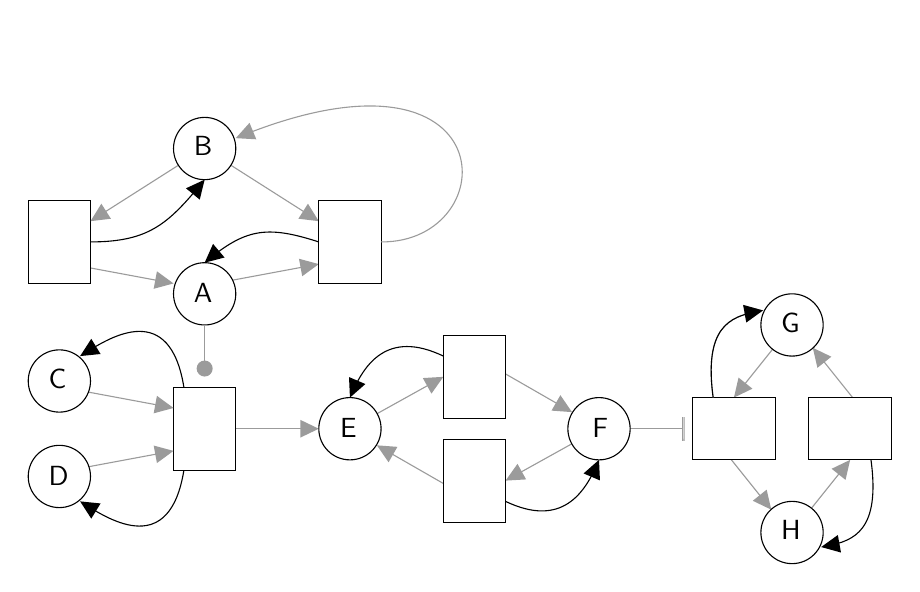
\begin{tikzpicture}[x=0.75pt,y=0.75pt,yscale=-1,xscale=1]
%uncomment if require: \path (0,300); %set diagram left start at 0, and has height of 300

%Straight Lines [id:da9814975397164354] 
\draw [color={rgb, 255:red, 155; green, 155; blue, 155 }  ,draw opacity=1 ]   (408,230) -- (434.13,197.34) ;
\draw [shift={(436,195)}, rotate = 488.66] [fill={rgb, 255:red, 155; green, 155; blue, 155 }  ,fill opacity=1 ][line width=0.08]  [draw opacity=0] (8.93,-4.29) -- (0,0) -- (8.93,4.29) -- cycle    ;
%Straight Lines [id:da9406459969344991] 
\draw [color={rgb, 255:red, 155; green, 155; blue, 155 }  ,draw opacity=1 ]   (370,184) -- (396.13,216.66) ;
\draw [shift={(398,219)}, rotate = 231.34] [fill={rgb, 255:red, 155; green, 155; blue, 155 }  ,fill opacity=1 ][line width=0.08]  [draw opacity=0] (8.93,-4.29) -- (0,0) -- (8.93,4.29) -- cycle    ;
%Straight Lines [id:da567762566187695] 
\draw [color={rgb, 255:red, 155; green, 155; blue, 155 }  ,draw opacity=1 ]   (408,130) -- (381.87,162.66) ;
\draw [shift={(380,165)}, rotate = 308.65999999999997] [fill={rgb, 255:red, 155; green, 155; blue, 155 }  ,fill opacity=1 ][line width=0.08]  [draw opacity=0] (8.93,-4.29) -- (0,0) -- (8.93,4.29) -- cycle    ;
%Straight Lines [id:da8407631771019597] 
\draw [color={rgb, 255:red, 155; green, 155; blue, 155 }  ,draw opacity=1 ]   (446,176) -- (419.87,143.34) ;
\draw [shift={(418,141)}, rotate = 411.34000000000003] [fill={rgb, 255:red, 155; green, 155; blue, 155 }  ,fill opacity=1 ][line width=0.08]  [draw opacity=0] (8.93,-4.29) -- (0,0) -- (8.93,4.29) -- cycle    ;
%Straight Lines [id:da18886988900572765] 
\draw [color={rgb, 255:red, 155; green, 155; blue, 155 }  ,draw opacity=1 ]   (315,180) -- (355,180) ;
%Straight Lines [id:da3931805508956303] 
\draw [color={rgb, 255:red, 155; green, 155; blue, 155 }  ,draw opacity=1 ]   (130,180) -- (177,180) ;
\draw [shift={(180,180)}, rotate = 180] [fill={rgb, 255:red, 155; green, 155; blue, 155 }  ,fill opacity=1 ][line width=0.08]  [draw opacity=0] (8.93,-4.29) -- (0,0) -- (8.93,4.29) -- cycle    ;
%Straight Lines [id:da8295871618343293] 
\draw [color={rgb, 255:red, 155; green, 155; blue, 155 }  ,draw opacity=1 ]   (255,145) -- (299.4,170.51) ;
\draw [shift={(302,172)}, rotate = 209.88] [fill={rgb, 255:red, 155; green, 155; blue, 155 }  ,fill opacity=1 ][line width=0.08]  [draw opacity=0] (8.93,-4.29) -- (0,0) -- (8.93,4.29) -- cycle    ;
%Straight Lines [id:da5331508184397238] 
\draw [color={rgb, 255:red, 155; green, 155; blue, 155 }  ,draw opacity=1 ]   (255,215) -- (210.6,189.49) ;
\draw [shift={(208,188)}, rotate = 389.88] [fill={rgb, 255:red, 155; green, 155; blue, 155 }  ,fill opacity=1 ][line width=0.08]  [draw opacity=0] (8.93,-4.29) -- (0,0) -- (8.93,4.29) -- cycle    ;
%Straight Lines [id:da9986006782985726] 
\draw [color={rgb, 255:red, 155; green, 155; blue, 155 }  ,draw opacity=1 ]   (315,180) -- (272.62,203.54) ;
\draw [shift={(270,205)}, rotate = 330.95] [fill={rgb, 255:red, 155; green, 155; blue, 155 }  ,fill opacity=1 ][line width=0.08]  [draw opacity=0] (8.93,-4.29) -- (0,0) -- (8.93,4.29) -- cycle    ;
%Straight Lines [id:da12348680583129257] 
\draw [color={rgb, 255:red, 155; green, 155; blue, 155 }  ,draw opacity=1 ]   (195,180) -- (237.38,156.46) ;
\draw [shift={(240,155)}, rotate = 510.95] [fill={rgb, 255:red, 155; green, 155; blue, 155 }  ,fill opacity=1 ][line width=0.08]  [draw opacity=0] (8.93,-4.29) -- (0,0) -- (8.93,4.29) -- cycle    ;
%Straight Lines [id:da9418451865861617] 
\draw [color={rgb, 255:red, 155; green, 155; blue, 155 }  ,draw opacity=1 ]   (130,110) -- (177.05,101.23) ;
\draw [shift={(180,100.68)}, rotate = 529.44] [fill={rgb, 255:red, 155; green, 155; blue, 155 }  ,fill opacity=1 ][line width=0.08]  [draw opacity=0] (8.93,-4.29) -- (0,0) -- (8.93,4.29) -- cycle    ;
%Straight Lines [id:da4404755375642728] 
\draw [color={rgb, 255:red, 155; green, 155; blue, 155 }  ,draw opacity=1 ]   (60,100.68) -- (107.05,109.45) ;
\draw [shift={(110,110)}, rotate = 190.56] [fill={rgb, 255:red, 155; green, 155; blue, 155 }  ,fill opacity=1 ][line width=0.08]  [draw opacity=0] (8.93,-4.29) -- (0,0) -- (8.93,4.29) -- cycle    ;
%Straight Lines [id:da30142710216357527] 
\draw [color={rgb, 255:red, 155; green, 155; blue, 155 }  ,draw opacity=1 ]   (125,45) -- (177.47,78.39) ;
\draw [shift={(180,80)}, rotate = 212.47] [fill={rgb, 255:red, 155; green, 155; blue, 155 }  ,fill opacity=1 ][line width=0.08]  [draw opacity=0] (8.93,-4.29) -- (0,0) -- (8.93,4.29) -- cycle    ;
%Shape: Rectangle [id:dp08787765148447635] 
\draw  [fill={rgb, 255:red, 255; green, 255; blue, 255 }  ,fill opacity=1 ] (40,70) -- (70,70) -- (70,110) -- (40,110) -- cycle ;
%Straight Lines [id:da003675026654497149] 
\draw [color={rgb, 255:red, 155; green, 155; blue, 155 }  ,draw opacity=1 ]   (125,45) -- (72.53,78.39) ;
\draw [shift={(70,80)}, rotate = 327.53] [fill={rgb, 255:red, 155; green, 155; blue, 155 }  ,fill opacity=1 ][line width=0.08]  [draw opacity=0] (8.93,-4.29) -- (0,0) -- (8.93,4.29) -- cycle    ;
%Shape: Circle [id:dp857493257636351] 
\draw  [fill={rgb, 255:red, 255; green, 255; blue, 255 }  ,fill opacity=1 ] (110,45) .. controls (110,36.72) and (116.72,30) .. (125,30) .. controls (133.28,30) and (140,36.72) .. (140,45) .. controls (140,53.28) and (133.28,60) .. (125,60) .. controls (116.72,60) and (110,53.28) .. (110,45) -- cycle ;
%Shape: Rectangle [id:dp06861100107998075] 
\draw  [fill={rgb, 255:red, 255; green, 255; blue, 255 }  ,fill opacity=1 ] (180,70) -- (210,70) -- (210,110) -- (180,110) -- cycle ;
%Curve Lines [id:da16899155142836797] 
\draw [color={rgb, 255:red, 155; green, 155; blue, 155 }  ,draw opacity=1 ]   (210,90) .. controls (270.06,90.4) and (270.75,-12.96) .. (141.95,39.2) ;
\draw [shift={(140,40)}, rotate = 337.56] [fill={rgb, 255:red, 155; green, 155; blue, 155 }  ,fill opacity=1 ][line width=0.08]  [draw opacity=0] (8.93,-4.29) -- (0,0) -- (8.93,4.29) -- cycle    ;
%Shape: Circle [id:dp6562288539389132] 
\draw  [fill={rgb, 255:red, 255; green, 255; blue, 255 }  ,fill opacity=1 ] (110,115) .. controls (110,106.72) and (116.72,100) .. (125,100) .. controls (133.28,100) and (140,106.72) .. (140,115) .. controls (140,123.28) and (133.28,130) .. (125,130) .. controls (116.72,130) and (110,123.28) .. (110,115) -- cycle ;
%Straight Lines [id:da5109350748561536] 
\draw [color={rgb, 255:red, 155; green, 155; blue, 155 }  ,draw opacity=1 ]   (125,130) -- (125,151) ;
\draw [shift={(125,151)}, rotate = 90] [color={rgb, 255:red, 155; green, 155; blue, 155 }  ,draw opacity=1 ][fill={rgb, 255:red, 155; green, 155; blue, 155 }  ,fill opacity=1 ][line width=0.75]      (0, 0) circle [x radius= 3.35, y radius= 3.35]   ;
%Shape: Rectangle [id:dp023984567760534814] 
\draw  [fill={rgb, 255:red, 255; green, 255; blue, 255 }  ,fill opacity=1 ] (110,160) -- (140,160) -- (140,200) -- (110,200) -- cycle ;
%Straight Lines [id:da035236663145903346] 
\draw [color={rgb, 255:red, 155; green, 155; blue, 155 }  ,draw opacity=1 ]   (60,160.68) -- (107.05,169.45) ;
\draw [shift={(110,170)}, rotate = 190.56] [fill={rgb, 255:red, 155; green, 155; blue, 155 }  ,fill opacity=1 ][line width=0.08]  [draw opacity=0] (8.93,-4.29) -- (0,0) -- (8.93,4.29) -- cycle    ;
%Straight Lines [id:da81539224069834] 
\draw [color={rgb, 255:red, 155; green, 155; blue, 155 }  ,draw opacity=1 ]   (60,200) -- (107.05,191.23) ;
\draw [shift={(110,190.68)}, rotate = 529.44] [fill={rgb, 255:red, 155; green, 155; blue, 155 }  ,fill opacity=1 ][line width=0.08]  [draw opacity=0] (8.93,-4.29) -- (0,0) -- (8.93,4.29) -- cycle    ;
%Shape: Circle [id:dp9606958833911112] 
\draw  [fill={rgb, 255:red, 255; green, 255; blue, 255 }  ,fill opacity=1 ] (40,157) .. controls (40,148.72) and (46.72,142) .. (55,142) .. controls (63.28,142) and (70,148.72) .. (70,157) .. controls (70,165.28) and (63.28,172) .. (55,172) .. controls (46.72,172) and (40,165.28) .. (40,157) -- cycle ;
%Shape: Circle [id:dp05257334197950425] 
\draw  [fill={rgb, 255:red, 255; green, 255; blue, 255 }  ,fill opacity=1 ] (40,203) .. controls (40,194.72) and (46.72,188) .. (55,188) .. controls (63.28,188) and (70,194.72) .. (70,203) .. controls (70,211.28) and (63.28,218) .. (55,218) .. controls (46.72,218) and (40,211.28) .. (40,203) -- cycle ;
%Shape: Circle [id:dp1512689330320689] 
\draw  [fill={rgb, 255:red, 255; green, 255; blue, 255 }  ,fill opacity=1 ] (180,180) .. controls (180,171.72) and (186.72,165) .. (195,165) .. controls (203.28,165) and (210,171.72) .. (210,180) .. controls (210,188.28) and (203.28,195) .. (195,195) .. controls (186.72,195) and (180,188.28) .. (180,180) -- cycle ;
%Shape: Rectangle [id:dp1719311079425654] 
\draw  [fill={rgb, 255:red, 255; green, 255; blue, 255 }  ,fill opacity=1 ] (240,135) -- (270,135) -- (270,175) -- (240,175) -- cycle ;
%Shape: Rectangle [id:dp029118782750540584] 
\draw  [fill={rgb, 255:red, 255; green, 255; blue, 255 }  ,fill opacity=1 ] (240,185) -- (270,185) -- (270,225) -- (240,225) -- cycle ;
%Shape: Circle [id:dp8904310206501505] 
\draw  [fill={rgb, 255:red, 255; green, 255; blue, 255 }  ,fill opacity=1 ] (300,180) .. controls (300,171.72) and (306.72,165) .. (315,165) .. controls (323.28,165) and (330,171.72) .. (330,180) .. controls (330,188.28) and (323.28,195) .. (315,195) .. controls (306.72,195) and (300,188.28) .. (300,180) -- cycle ;
%Straight Lines [id:da781554004447597] 
\draw [color={rgb, 255:red, 155; green, 155; blue, 155 }  ,draw opacity=1 ]   (355.29,174.43) -- (355.26,185.81) ;
%Straight Lines [id:da7582574980289809] 
\draw [color={rgb, 255:red, 155; green, 155; blue, 155 }  ,draw opacity=1 ]   (356,174.43) -- (355.97,185.81) ;
%Shape: Rectangle [id:dp3426485498076772] 
\draw  [fill={rgb, 255:red, 255; green, 255; blue, 255 }  ,fill opacity=1 ] (400,165) -- (400,195) -- (360,195) -- (360,165) -- cycle ;
%Shape: Rectangle [id:dp6338678858875948] 
\draw  [fill={rgb, 255:red, 255; green, 255; blue, 255 }  ,fill opacity=1 ] (456,165) -- (456,195) -- (416,195) -- (416,165) -- cycle ;
%Shape: Circle [id:dp12073790053942313] 
\draw  [fill={rgb, 255:red, 255; green, 255; blue, 255 }  ,fill opacity=1 ] (393,130) .. controls (393,121.72) and (399.72,115) .. (408,115) .. controls (416.28,115) and (423,121.72) .. (423,130) .. controls (423,138.28) and (416.28,145) .. (408,145) .. controls (399.72,145) and (393,138.28) .. (393,130) -- cycle ;
%Shape: Circle [id:dp533012533964861] 
\draw  [fill={rgb, 255:red, 255; green, 255; blue, 255 }  ,fill opacity=1 ] (393,230) .. controls (393,221.72) and (399.72,215) .. (408,215) .. controls (416.28,215) and (423,221.72) .. (423,230) .. controls (423,238.28) and (416.28,245) .. (408,245) .. controls (399.72,245) and (393,238.28) .. (393,230) -- cycle ;
%Curve Lines [id:da884601900599596] 
\draw    (70,90) .. controls (97.73,89.97) and (107.08,81.59) .. (123.22,62.16) ;
\draw [shift={(125,60)}, rotate = 489.47] [fill={rgb, 255:red, 0; green, 0; blue, 0 }  ][line width=0.08]  [draw opacity=0] (8.93,-4.29) -- (0,0) -- (8.93,4.29) -- cycle    ;
%Curve Lines [id:da47207162896041743] 
\draw    (180,90) .. controls (155.94,82.25) and (145.47,83.22) .. (127.04,98.3) ;
\draw [shift={(125,100)}, rotate = 319.76] [fill={rgb, 255:red, 0; green, 0; blue, 0 }  ][line width=0.08]  [draw opacity=0] (8.93,-4.29) -- (0,0) -- (8.93,4.29) -- cycle    ;
%Curve Lines [id:da6901431067530599] 
\draw    (115,160) .. controls (108.24,118.12) and (79.8,135.66) .. (67.49,143.44) ;
\draw [shift={(65,145)}, rotate = 328.53] [fill={rgb, 255:red, 0; green, 0; blue, 0 }  ][line width=0.08]  [draw opacity=0] (8.93,-4.29) -- (0,0) -- (8.93,4.29) -- cycle    ;
%Curve Lines [id:da5177921743405851] 
\draw    (115,200) .. controls (108.24,241.88) and (79.8,224.34) .. (67.49,216.56) ;
\draw [shift={(65,215)}, rotate = 391.47] [fill={rgb, 255:red, 0; green, 0; blue, 0 }  ][line width=0.08]  [draw opacity=0] (8.93,-4.29) -- (0,0) -- (8.93,4.29) -- cycle    ;
%Curve Lines [id:da5942699000639224] 
\draw    (240,145) .. controls (212.64,131.88) and (201.82,149.68) .. (196.12,162.43) ;
\draw [shift={(195,165)}, rotate = 293.04] [fill={rgb, 255:red, 0; green, 0; blue, 0 }  ][line width=0.08]  [draw opacity=0] (8.93,-4.29) -- (0,0) -- (8.93,4.29) -- cycle    ;
%Curve Lines [id:da15566992900671806] 
\draw    (270,215) .. controls (297.36,228.12) and (308.18,210.32) .. (313.88,197.57) ;
\draw [shift={(315,195)}, rotate = 473.04] [fill={rgb, 255:red, 0; green, 0; blue, 0 }  ][line width=0.08]  [draw opacity=0] (8.93,-4.29) -- (0,0) -- (8.93,4.29) -- cycle    ;
%Curve Lines [id:da15566992900671806] 
\draw [color={rgb, 255:red, 155; green, 155; blue, 155 }  ,draw opacity=1 ]   (370,165) .. controls (365.41,131.05) and (378.06,126.08) .. (391.07,123.54) ;
\draw [shift={(394,123)}, rotate = 529.8299999999999] [fill={rgb, 255:red, 155; green, 155; blue, 155 }  ,fill opacity=1 ][line width=0.08]  [draw opacity=0] (8.93,-4.29) -- (0,0) -- (8.93,4.29) -- cycle    ;
%Curve Lines [id:da21250749688448223] 
\draw [color={rgb, 255:red, 0; green, 0; blue, 0 }  ,draw opacity=1 ]   (446.04,195) .. controls (450.63,228.95) and (437.98,233.92) .. (424.97,236.46) ;
\draw [shift={(422.04,237)}, rotate = 349.83000000000004] [fill={rgb, 255:red, 0; green, 0; blue, 0 }  ,fill opacity=1 ][line width=0.08]  [draw opacity=0] (8.93,-4.29) -- (0,0) -- (8.93,4.29) -- cycle    ;
%Curve Lines [id:da8896510092620566] 
\draw [color={rgb, 255:red, 0; green, 0; blue, 0 }  ,draw opacity=1 ]   (370,165) .. controls (365.41,131.05) and (378.06,126.08) .. (391.07,123.54) ;
\draw [shift={(394,123)}, rotate = 529.8299999999999] [fill={rgb, 255:red, 0; green, 0; blue, 0 }  ,fill opacity=1 ][line width=0.08]  [draw opacity=0] (8.93,-4.29) -- (0,0) -- (8.93,4.29) -- cycle    ;


% Text Node
\draw (118.5,38) node [anchor=north west][inner sep=0.75pt]   [align=left] {$\mathsf{B}$};
% Text Node
\draw (118.5,108.5) node [anchor=north west][inner sep=0.75pt]   [align=left] {$\mathsf{A}$};
% Text Node
\draw (48.5,150) node [anchor=north west][inner sep=0.75pt]   [align=left] {$\mathsf{C}$};
% Text Node
\draw (48.5,197) node [anchor=north west][inner sep=0.75pt]   [align=left] {$\mathsf{D}$};
% Text Node
\draw (189,173.5) node [anchor=north west][inner sep=0.75pt]   [align=left] {$\mathsf{E}$};
% Text Node
\draw (310.5,173.5) node [anchor=north west][inner sep=0.75pt]   [align=left] {$\mathsf{F}$};
% Text Node
\draw (401.5,123) node [anchor=north west][inner sep=0.75pt]   [align=left] {$\mathsf{G}$};
% Text Node
\draw (401.5,223) node [anchor=north west][inner sep=0.75pt]   [align=left] {$\mathsf{H}$};


\end{tikzpicture}}
    \caption{The enriched pathway graph obtained from the pathway graph of Figure \ref{fig:pathway-graph}. The edges added with respect to the original graph are shown in black.}
    \label{fig:pathway-graph-enriched}
\end{figure*}
The purpose of the enriched pathway graph is to determine which portion of the associated pathway graph is relevant for the assessment of the robustness. With the help of the enriched graph $G'$, we can introduce the subgraph of $G$ induced by an input pair ($\mathsf{I},\mathsf{O}$) as a graph $S_{\mathsf{I},\mathsf{O}} = \Tuple{\Cal{V}_{S_{\mathsf{I},\mathsf{O}}}, \Cal{E}_{S_{\mathsf{I},\mathsf{O}}}}$, defined informally as follows: $S_{\mathsf{I},\mathsf{O}}$ is the smallest subgraph of $G$ whose node set contains $\mathsf{I}$, $\mathsf{O}$, as well as nodes in every possible oriented path from $\mathsf{I}$ to $\mathsf{O}$ in $G'$. We remark that $S_{\mathsf{I},\mathsf{O}}$ is a subgraph of $G$, although its node set is computed on the basis of the paths in $G'$. Figure \ref{fig:subgraphs} shows some examples of induced subgraphs extracted from the graph in Figure \ref{fig:pathway-graph}.
\begin{figure*}[h!]
    \begin{subfigure}[b]{0.24\linewidth}
        \centering
        \resizebox{.9\textwidth}{!}{

\tikzset{every picture/.style={line width=0.75pt}} %set default line width to 0.75pt

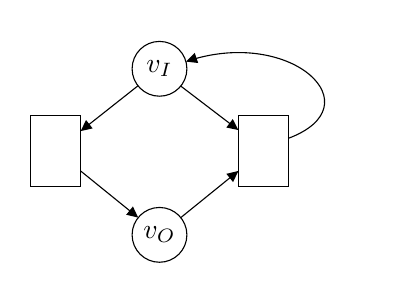
\begin{tikzpicture}[x=0.75pt,y=0.75pt,yscale=-1,xscale=1]
%uncomment if require: \path (0,200); %set diagram left start at 0, and has height of 200

%Straight Lines [id:da5988806727183245]
\draw    (120,76) -- (155.62,103.18) ;
\draw [shift={(158,105)}, rotate = 217.35] [fill={rgb, 255:red, 0; green, 0; blue, 0 }  ][line width=0.08]  [draw opacity=0] (5.36,-2.57) -- (0,0) -- (5.36,2.57) -- cycle    ;

% Text Node
\draw  [fill={rgb, 255:red, 255; green, 255; blue, 255 }  ,fill opacity=1 ]  (58,98) -- (82,98) -- (82,132) -- (58,132) -- cycle  ;
\draw (70,115) node   [align=left] {\begin{minipage}[lt]{13.600000000000001pt}\setlength\topsep{0pt}
\begin{center}
\end{center}

\end{minipage}};
% Text Node
\draw  [fill={rgb, 255:red, 255; green, 255; blue, 255 }  ,fill opacity=1 ]  (120, 75.5) circle [x radius= 13.2, y radius= 13.2]   ;
\draw (120,75.5) node   [align=left] {\begin{minipage}[lt]{14.96pt}\setlength\topsep{0pt}
\begin{center}
$\displaystyle v_{I}$
\end{center}

\end{minipage}};
% Text Node
\draw  [fill={rgb, 255:red, 255; green, 255; blue, 255 }  ,fill opacity=1 ]  (158,98) -- (182,98) -- (182,132) -- (158,132) -- cycle  ;
\draw (170,115) node   [align=left] {\begin{minipage}[lt]{13.600000000000001pt}\setlength\topsep{0pt}
\begin{center}
\end{center}

\end{minipage}};
% Text Node
\draw  [fill={rgb, 255:red, 255; green, 255; blue, 255 }  ,fill opacity=1 ]  (120, 155.5) circle [x radius= 13.2, y radius= 13.2]   ;
\draw (120,155.5) node   [align=left] {\begin{minipage}[lt]{14.96pt}\setlength\topsep{0pt}
\begin{center}
$\displaystyle v_{O}$
\end{center}

\end{minipage}};
% Connection
\draw    (109.64,83.68) -- (84.35,103.66) ;
\draw [shift={(82,105.52)}, rotate = 321.69] [fill={rgb, 255:red, 0; green, 0; blue, 0 }  ][line width=0.08]  [draw opacity=0] (5.36,-2.57) -- (0,0) -- (5.36,2.57) -- cycle    ;
% Connection
\draw    (82,124.72) -- (107.41,145.3) ;
\draw [shift={(109.74,147.19)}, rotate = 219.01] [fill={rgb, 255:red, 0; green, 0; blue, 0 }  ][line width=0.08]  [draw opacity=0] (5.36,-2.57) -- (0,0) -- (5.36,2.57) -- cycle    ;
% Connection
\draw    (130.26,147.19) -- (155.67,126.61) ;
\draw [shift={(158,124.72)}, rotate = 500.99] [fill={rgb, 255:red, 0; green, 0; blue, 0 }  ][line width=0.08]  [draw opacity=0] (5.36,-2.57) -- (0,0) -- (5.36,2.57) -- cycle    ;
% Connection
\draw    (182,109.03) .. controls (223.8,93.44) and (184.07,55.95) .. (134.99,71.28) ;
\draw [shift={(132.74,72.02)}, rotate = 341.03] [fill={rgb, 255:red, 0; green, 0; blue, 0 }  ][line width=0.08]  [draw opacity=0] (5.36,-2.57) -- (0,0) -- (5.36,2.57) -- cycle    ;

\end{tikzpicture}}
        \caption{$\mathsf{I}=\mathsf{B},\, \mathsf{O}=\mathsf{A}$}\label{subfig:subgraph1}
    \end{subfigure}
    %
    \begin{subfigure}[b]{0.29\linewidth}
        \centering
        \resizebox{.9\textwidth}{!}{

\tikzset{every picture/.style={line width=0.75pt}} %set default line width to 0.75pt

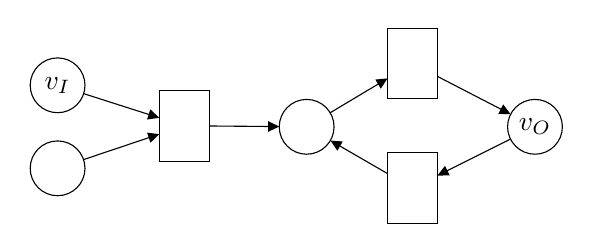
\begin{tikzpicture}[x=0.75pt,y=0.75pt,yscale=-1,xscale=1]
%uncomment if require: \path (0,128); %set diagram left start at 0, and has height of 128


% Text Node
\draw  [fill={rgb, 255:red, 255; green, 255; blue, 255 }  ,fill opacity=1 ]  (29, 41) circle [x radius= 13.2, y radius= 13.2]   ;
\draw (29,41) node   [align=left] {\begin{minipage}[lt]{14.96pt}\setlength\topsep{0pt}
\begin{center}
$\displaystyle v_{I}$
\end{center}

\end{minipage}};
% Text Node
\draw  [fill={rgb, 255:red, 255; green, 255; blue, 255 }  ,fill opacity=1 ]  (29, 81) circle [x radius= 13.2, y radius= 13.2]   ;
\draw (29,81) node   [align=left] {\begin{minipage}[lt]{14.96pt}\setlength\topsep{0pt}
\begin{center}
\end{center}

\end{minipage}};
% Text Node
\draw  [fill={rgb, 255:red, 255; green, 255; blue, 255 }  ,fill opacity=1 ]  (78,43.5) -- (102,43.5) -- (102,77.5) -- (78,77.5) -- cycle  ;
\draw (90,60.5) node   [align=left] {\begin{minipage}[lt]{13.600000000000001pt}\setlength\topsep{0pt}
\begin{center}
\end{center}

\end{minipage}};
% Text Node
\draw  [fill={rgb, 255:red, 255; green, 255; blue, 255 }  ,fill opacity=1 ]  (149, 61) circle [x radius= 13.2, y radius= 13.2]   ;
\draw (149,61) node   [align=left] {\begin{minipage}[lt]{14.96pt}\setlength\topsep{0pt}
\begin{center}
\end{center}

\end{minipage}};
% Text Node
\draw  [fill={rgb, 255:red, 255; green, 255; blue, 255 }  ,fill opacity=1 ]  (188,13.5) -- (212,13.5) -- (212,47.5) -- (188,47.5) -- cycle  ;
\draw (200,30.5) node   [align=left] {\begin{minipage}[lt]{13.600000000000001pt}\setlength\topsep{0pt}
\begin{center}
\end{center}

\end{minipage}};
% Text Node
\draw  [fill={rgb, 255:red, 255; green, 255; blue, 255 }  ,fill opacity=1 ]  (188,73.5) -- (212,73.5) -- (212,107.5) -- (188,107.5) -- cycle  ;
\draw (200,90.5) node   [align=left] {\begin{minipage}[lt]{13.600000000000001pt}\setlength\topsep{0pt}
\begin{center}
\end{center}

\end{minipage}};
% Text Node
\draw  [fill={rgb, 255:red, 255; green, 255; blue, 255 }  ,fill opacity=1 ]  (259, 61) circle [x radius= 13.2, y radius= 13.2]   ;
\draw (259,61) node   [align=left] {\begin{minipage}[lt]{14.96pt}\setlength\topsep{0pt}
\begin{center}
$\displaystyle v_{O}$
\end{center}

\end{minipage}};
% Connection
\draw    (41.58,45.02) -- (75.14,55.75) ;
\draw [shift={(78,56.66)}, rotate = 197.73] [fill={rgb, 255:red, 0; green, 0; blue, 0 }  ][line width=0.08]  [draw opacity=0] (5.36,-2.57) -- (0,0) -- (5.36,2.57) -- cycle    ;
% Connection
\draw    (41.52,76.79) -- (75.16,65.49) ;
\draw [shift={(78,64.53)}, rotate = 521.4200000000001] [fill={rgb, 255:red, 0; green, 0; blue, 0 }  ][line width=0.08]  [draw opacity=0] (5.36,-2.57) -- (0,0) -- (5.36,2.57) -- cycle    ;
% Connection
\draw    (102,60.6) -- (132.8,60.86) ;
\draw [shift={(135.8,60.89)}, rotate = 180.49] [fill={rgb, 255:red, 0; green, 0; blue, 0 }  ][line width=0.08]  [draw opacity=0] (5.36,-2.57) -- (0,0) -- (5.36,2.57) -- cycle    ;
% Connection
\draw    (160.33,54.22) -- (185.43,39.22) ;
\draw [shift={(188,37.68)}, rotate = 509.12] [fill={rgb, 255:red, 0; green, 0; blue, 0 }  ][line width=0.08]  [draw opacity=0] (5.36,-2.57) -- (0,0) -- (5.36,2.57) -- cycle    ;
% Connection
\draw    (212,36.7) -- (244.61,53.56) ;
\draw [shift={(247.27,54.94)}, rotate = 207.34] [fill={rgb, 255:red, 0; green, 0; blue, 0 }  ][line width=0.08]  [draw opacity=0] (5.36,-2.57) -- (0,0) -- (5.36,2.57) -- cycle    ;
% Connection
\draw    (247.19,66.9) -- (214.68,83.16) ;
\draw [shift={(212,84.5)}, rotate = 333.43] [fill={rgb, 255:red, 0; green, 0; blue, 0 }  ][line width=0.08]  [draw opacity=0] (5.36,-2.57) -- (0,0) -- (5.36,2.57) -- cycle    ;
% Connection
\draw    (188,83.56) -- (163.03,69.11) ;
\draw [shift={(160.43,67.61)}, rotate = 390.05] [fill={rgb, 255:red, 0; green, 0; blue, 0 }  ][line width=0.08]  [draw opacity=0] (5.36,-2.57) -- (0,0) -- (5.36,2.57) -- cycle    ;

\end{tikzpicture}}
        \caption{$\mathsf{I}=\mathsf{C},\, \mathsf{O}=\mathsf{F}$}\label{subfig:subgraph2}
    \end{subfigure}
    %
    \begin{subfigure}[b]{0.44\linewidth}
        \centering
        \resizebox{.9\textwidth}{!}{

\tikzset{every picture/.style={line width=0.75pt}} %set default line width to 0.75pt        

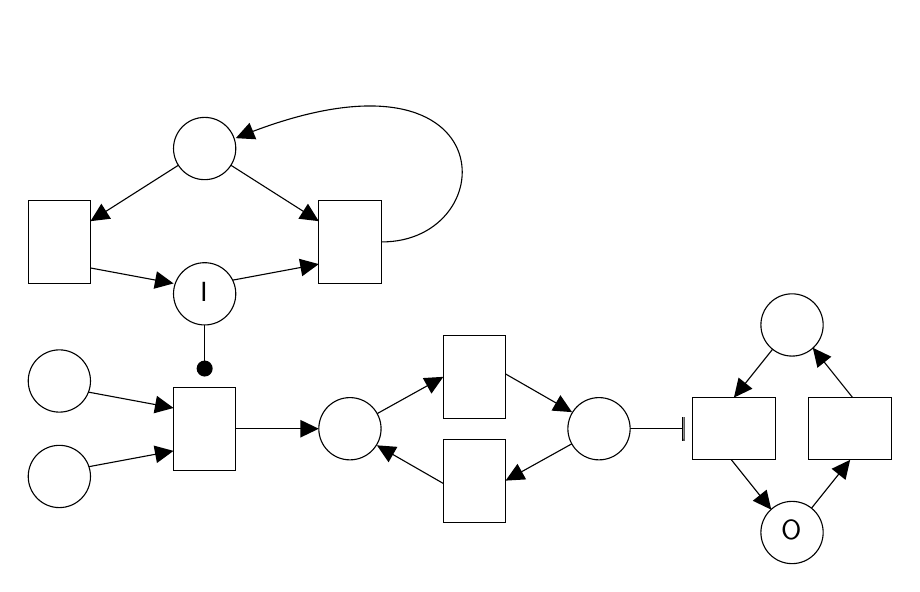
\begin{tikzpicture}[x=0.75pt,y=0.75pt,yscale=-1,xscale=1]
%uncomment if require: \path (0,263); %set diagram left start at 0, and has height of 263

%Straight Lines [id:da9076248721928286] 
\draw    (408,230) -- (434.13,197.34) ;
\draw [shift={(436,195)}, rotate = 488.66] [fill={rgb, 255:red, 0; green, 0; blue, 0 }  ][line width=0.08]  [draw opacity=0] (8.93,-4.29) -- (0,0) -- (8.93,4.29) -- cycle    ;
%Straight Lines [id:da8310282669133191] 
\draw    (370,184) -- (396.13,216.66) ;
\draw [shift={(398,219)}, rotate = 231.34] [fill={rgb, 255:red, 0; green, 0; blue, 0 }  ][line width=0.08]  [draw opacity=0] (8.93,-4.29) -- (0,0) -- (8.93,4.29) -- cycle    ;
%Straight Lines [id:da21056116046945594] 
\draw    (408,130) -- (381.87,162.66) ;
\draw [shift={(380,165)}, rotate = 308.65999999999997] [fill={rgb, 255:red, 0; green, 0; blue, 0 }  ][line width=0.08]  [draw opacity=0] (8.93,-4.29) -- (0,0) -- (8.93,4.29) -- cycle    ;
%Straight Lines [id:da5752373273055789] 
\draw    (446,176) -- (419.87,143.34) ;
\draw [shift={(418,141)}, rotate = 411.34000000000003] [fill={rgb, 255:red, 0; green, 0; blue, 0 }  ][line width=0.08]  [draw opacity=0] (8.93,-4.29) -- (0,0) -- (8.93,4.29) -- cycle    ;
%Straight Lines [id:da16579110027769128] 
\draw    (315,180) -- (355,180) ;
%Straight Lines [id:da4838109924037106] 
\draw    (130,180) -- (177,180) ;
\draw [shift={(180,180)}, rotate = 180] [fill={rgb, 255:red, 0; green, 0; blue, 0 }  ][line width=0.08]  [draw opacity=0] (8.93,-4.29) -- (0,0) -- (8.93,4.29) -- cycle    ;
%Straight Lines [id:da1725280869298207] 
\draw    (255,145) -- (299.4,170.51) ;
\draw [shift={(302,172)}, rotate = 209.88] [fill={rgb, 255:red, 0; green, 0; blue, 0 }  ][line width=0.08]  [draw opacity=0] (8.93,-4.29) -- (0,0) -- (8.93,4.29) -- cycle    ;
%Straight Lines [id:da34654117341962776] 
\draw    (255,215) -- (210.6,189.49) ;
\draw [shift={(208,188)}, rotate = 389.88] [fill={rgb, 255:red, 0; green, 0; blue, 0 }  ][line width=0.08]  [draw opacity=0] (8.93,-4.29) -- (0,0) -- (8.93,4.29) -- cycle    ;
%Straight Lines [id:da2572335252881772] 
\draw    (315,180) -- (272.62,203.54) ;
\draw [shift={(270,205)}, rotate = 330.95] [fill={rgb, 255:red, 0; green, 0; blue, 0 }  ][line width=0.08]  [draw opacity=0] (8.93,-4.29) -- (0,0) -- (8.93,4.29) -- cycle    ;
%Straight Lines [id:da9569901142124524] 
\draw    (195,180) -- (237.38,156.46) ;
\draw [shift={(240,155)}, rotate = 510.95] [fill={rgb, 255:red, 0; green, 0; blue, 0 }  ][line width=0.08]  [draw opacity=0] (8.93,-4.29) -- (0,0) -- (8.93,4.29) -- cycle    ;
%Straight Lines [id:da920112653947581] 
\draw    (130,110) -- (177.05,101.23) ;
\draw [shift={(180,100.68)}, rotate = 529.44] [fill={rgb, 255:red, 0; green, 0; blue, 0 }  ][line width=0.08]  [draw opacity=0] (8.93,-4.29) -- (0,0) -- (8.93,4.29) -- cycle    ;
%Straight Lines [id:da7419253152894756] 
\draw    (60,100.68) -- (107.05,109.45) ;
\draw [shift={(110,110)}, rotate = 190.56] [fill={rgb, 255:red, 0; green, 0; blue, 0 }  ][line width=0.08]  [draw opacity=0] (8.93,-4.29) -- (0,0) -- (8.93,4.29) -- cycle    ;
%Straight Lines [id:da9584629103768068] 
\draw    (125,45) -- (177.47,78.39) ;
\draw [shift={(180,80)}, rotate = 212.47] [fill={rgb, 255:red, 0; green, 0; blue, 0 }  ][line width=0.08]  [draw opacity=0] (8.93,-4.29) -- (0,0) -- (8.93,4.29) -- cycle    ;
%Shape: Rectangle [id:dp7470169028080813] 
\draw  [fill={rgb, 255:red, 255; green, 255; blue, 255 }  ,fill opacity=1 ] (40,70) -- (70,70) -- (70,110) -- (40,110) -- cycle ;
%Straight Lines [id:da7129571423389669] 
\draw    (125,45) -- (72.53,78.39) ;
\draw [shift={(70,80)}, rotate = 327.53] [fill={rgb, 255:red, 0; green, 0; blue, 0 }  ][line width=0.08]  [draw opacity=0] (8.93,-4.29) -- (0,0) -- (8.93,4.29) -- cycle    ;
%Shape: Circle [id:dp7911048844652653] 
\draw  [fill={rgb, 255:red, 255; green, 255; blue, 255 }  ,fill opacity=1 ] (110,45) .. controls (110,36.72) and (116.72,30) .. (125,30) .. controls (133.28,30) and (140,36.72) .. (140,45) .. controls (140,53.28) and (133.28,60) .. (125,60) .. controls (116.72,60) and (110,53.28) .. (110,45) -- cycle ;
%Shape: Rectangle [id:dp7683065667775133] 
\draw  [fill={rgb, 255:red, 255; green, 255; blue, 255 }  ,fill opacity=1 ] (180,70) -- (210,70) -- (210,110) -- (180,110) -- cycle ;
%Curve Lines [id:da44464433303214457] 
\draw    (210,90) .. controls (270.06,90.4) and (270.75,-12.96) .. (141.95,39.2) ;
\draw [shift={(140,40)}, rotate = 337.56] [fill={rgb, 255:red, 0; green, 0; blue, 0 }  ][line width=0.08]  [draw opacity=0] (8.93,-4.29) -- (0,0) -- (8.93,4.29) -- cycle    ;
%Shape: Circle [id:dp6369849547820912] 
\draw  [fill={rgb, 255:red, 255; green, 255; blue, 255 }  ,fill opacity=1 ] (110,115) .. controls (110,106.72) and (116.72,100) .. (125,100) .. controls (133.28,100) and (140,106.72) .. (140,115) .. controls (140,123.28) and (133.28,130) .. (125,130) .. controls (116.72,130) and (110,123.28) .. (110,115) -- cycle ;
%Straight Lines [id:da8558653638989671] 
\draw    (125,130) -- (125,151) ;
\draw [shift={(125,151)}, rotate = 90] [color={rgb, 255:red, 0; green, 0; blue, 0 }  ][fill={rgb, 255:red, 0; green, 0; blue, 0 }  ][line width=0.75]      (0, 0) circle [x radius= 3.35, y radius= 3.35]   ;
%Shape: Rectangle [id:dp2555616169207473] 
\draw  [fill={rgb, 255:red, 255; green, 255; blue, 255 }  ,fill opacity=1 ] (110,160) -- (140,160) -- (140,200) -- (110,200) -- cycle ;
%Straight Lines [id:da025173975162050777] 
\draw    (60,160.68) -- (107.05,169.45) ;
\draw [shift={(110,170)}, rotate = 190.56] [fill={rgb, 255:red, 0; green, 0; blue, 0 }  ][line width=0.08]  [draw opacity=0] (8.93,-4.29) -- (0,0) -- (8.93,4.29) -- cycle    ;
%Straight Lines [id:da2606365706970364] 
\draw    (60,200) -- (107.05,191.23) ;
\draw [shift={(110,190.68)}, rotate = 529.44] [fill={rgb, 255:red, 0; green, 0; blue, 0 }  ][line width=0.08]  [draw opacity=0] (8.93,-4.29) -- (0,0) -- (8.93,4.29) -- cycle    ;
%Shape: Circle [id:dp04449919596066709] 
\draw  [fill={rgb, 255:red, 255; green, 255; blue, 255 }  ,fill opacity=1 ] (40,157) .. controls (40,148.72) and (46.72,142) .. (55,142) .. controls (63.28,142) and (70,148.72) .. (70,157) .. controls (70,165.28) and (63.28,172) .. (55,172) .. controls (46.72,172) and (40,165.28) .. (40,157) -- cycle ;
%Shape: Circle [id:dp22634666421190697] 
\draw  [fill={rgb, 255:red, 255; green, 255; blue, 255 }  ,fill opacity=1 ] (40,203) .. controls (40,194.72) and (46.72,188) .. (55,188) .. controls (63.28,188) and (70,194.72) .. (70,203) .. controls (70,211.28) and (63.28,218) .. (55,218) .. controls (46.72,218) and (40,211.28) .. (40,203) -- cycle ;
%Shape: Circle [id:dp8370082251852078] 
\draw  [fill={rgb, 255:red, 255; green, 255; blue, 255 }  ,fill opacity=1 ] (180,180) .. controls (180,171.72) and (186.72,165) .. (195,165) .. controls (203.28,165) and (210,171.72) .. (210,180) .. controls (210,188.28) and (203.28,195) .. (195,195) .. controls (186.72,195) and (180,188.28) .. (180,180) -- cycle ;
%Shape: Rectangle [id:dp939444556732205] 
\draw  [fill={rgb, 255:red, 255; green, 255; blue, 255 }  ,fill opacity=1 ] (240,135) -- (270,135) -- (270,175) -- (240,175) -- cycle ;
%Shape: Rectangle [id:dp6023598592965531] 
\draw  [fill={rgb, 255:red, 255; green, 255; blue, 255 }  ,fill opacity=1 ] (240,185) -- (270,185) -- (270,225) -- (240,225) -- cycle ;
%Shape: Circle [id:dp39166844545870805] 
\draw  [fill={rgb, 255:red, 255; green, 255; blue, 255 }  ,fill opacity=1 ] (300,180) .. controls (300,171.72) and (306.72,165) .. (315,165) .. controls (323.28,165) and (330,171.72) .. (330,180) .. controls (330,188.28) and (323.28,195) .. (315,195) .. controls (306.72,195) and (300,188.28) .. (300,180) -- cycle ;
%Straight Lines [id:da6302251066776063] 
\draw    (355.29,174.43) -- (355.26,185.81) ;
%Straight Lines [id:da09616421048913337] 
\draw    (356,174.43) -- (355.97,185.81) ;
%Shape: Rectangle [id:dp49358854050629763] 
\draw  [fill={rgb, 255:red, 255; green, 255; blue, 255 }  ,fill opacity=1 ] (400,165) -- (400,195) -- (360,195) -- (360,165) -- cycle ;
%Shape: Rectangle [id:dp10449510627567582] 
\draw  [fill={rgb, 255:red, 255; green, 255; blue, 255 }  ,fill opacity=1 ] (456,165) -- (456,195) -- (416,195) -- (416,165) -- cycle ;
%Shape: Circle [id:dp5901019515208137] 
\draw  [fill={rgb, 255:red, 255; green, 255; blue, 255 }  ,fill opacity=1 ] (393,130) .. controls (393,121.72) and (399.72,115) .. (408,115) .. controls (416.28,115) and (423,121.72) .. (423,130) .. controls (423,138.28) and (416.28,145) .. (408,145) .. controls (399.72,145) and (393,138.28) .. (393,130) -- cycle ;
%Shape: Circle [id:dp23856981879081252] 
\draw  [fill={rgb, 255:red, 255; green, 255; blue, 255 }  ,fill opacity=1 ] (393,230) .. controls (393,221.72) and (399.72,215) .. (408,215) .. controls (416.28,215) and (423,221.72) .. (423,230) .. controls (423,238.28) and (416.28,245) .. (408,245) .. controls (399.72,245) and (393,238.28) .. (393,230) -- cycle ;

% Text Node
\draw (121.5,108) node [anchor=north west][inner sep=0.75pt]   [align=left] {$\mathsf{I}$};
% Text Node
\draw (401.5,223) node [anchor=north west][inner sep=0.75pt]   [align=left] {$\mathsf{O}$};


\end{tikzpicture}}
        \caption{$\mathsf{I}=\mathsf{A},\, \mathsf{O}=\mathsf{H}$}\label{subfig:subgraph3}
    \end{subfigure}
    \caption{Examples of subgraphs of the pathway graph in Figure \ref{fig:pathway-graph} induced by different input/output node pairs $(\mathsf{I},\mathsf{O})$.}\label{fig:subgraphs}
\end{figure*}

\subsection{Robustness Computation}\label{sec:robustness-computation}
The robustness values used to label the induced subgraphs are computed following the relative $\alpha$-robustness approach. The dynamics of each biochemical pathway has been simulated by applying a numerical solver (the \texttt{libRoadRunner} Python library by \cite{somogyi2015libroadrunner}) to its ODEs representation. Reference initial concentrations of involved molecules have been obtained from the original SBML model of each pathway. Moreover, 100 simulations have been performed for each molecule, by perturbing its initial concentration in the range $[-20\%,+20\%]$. The termination of each simulation has been set to the achievement of the steady state, with a timeout of 250 simulated time units.\footnote{The concentration values obtained at the end of the simulation are considered as steady state values also in the cases in which a timeout has been reached.} Given a subgraph $S_{\mathsf{I}, \mathsf{O}}$, we computed the width $\alpha$ of the range of concentrations reached by the output molecules $\mathsf{O}$ by varying the input $\mathsf{I}$ (as per definition of $\alpha$-robustness). A relative robustness $\overline{\alpha}$ has then been obtained by dividing $\alpha$ by the concentration reached by the output when the initial concentration of the input is the reference one (no perturbation). The final robustness value $r_{\mathsf{I}, \mathsf{O}} \in [0,1]$ has been computed by comparing $\overline{\alpha}$ (a relative representation of the output range) with $0.4$ (a relative representation of the initial input range, that is $40\%$) as follows:
\[
    r_{\mathsf{I}, \mathsf{O}} = 1 - min (1,\frac{\overline{\alpha}}{0.4})
\]

\subsection{Data Preprocessing}\label{subsec:data-collection}
Our initial data collection consisted of 706 SBML models of biochemical pathways, downloaded from the BioModels database \cite{le2006biomodels}. Specifically, the data correspond to the complete set of manually curated models present in the database at the time we started the construction of the dataset\footnote{May 2019.}. We removed empty models (not containing any node) and discarded duplicates, reducing the number of SBML models to 484. These models were first transformed into \glspl{ppn} representations and saved in DOT format\footnote{The DOT graph description language specification, available at: \url{https://graphviz.gitlab.io/_pages/doc/info/lang.html}}. For the translation of the SMBL models into \glspl{ppn}, we developed a Python script that, for each reaction in the SMBL model extracts reactants, products and modifiers. Furthermore, it also checks the kinetic formula in order to determine whether each modifier is either promoter or an inhibitor. With the conversion of each \gls{ppn} into a pathway graph, we obtained a collection $\Cal{G} = \Set{G_i}_{i=1}^{484}$ of pathway graphs. Each of these pathway graphs has been transformed into a set containing one induced subgraph (whose size does not exceed 100 nodes, for computational reasons) for every possible input/output combination of pathway graph nodes representing molecules, according to the procedure detailed in Section \ref{sec:subgraphs-extraction}. For each induced subgraph, the associated robustness has been calculated as explained in Section \ref{sec:robustness-computation}. The result of this preprocessing is a training dataset:
$$\mathbb{G} = \bigcup\limits_{G \in \Cal{G}} \Set{(S_{\mathsf{I},\mathsf{O}}, \overline{r}_{{\mathsf{I},\mathsf{O}}}) \mid \forall (\mathsf{I},\mathsf{O}) \in \Cal{V}_{G}^{\Fun{mol}}},$$
where $\overline{r}_{\mathsf{I}, \mathsf{O}} = \mathbb{I}[r_{\mathsf{I}, \mathsf{O}} > 0.5]$ are robustness indicators used as the labels for the associated binary classification task. The total number of subgraphs in the preprocessed dataset is 44928.

\subsection{Subgraph Features}
We encoded information such as node type, edge type, and input/output pair of the induced subgraphs in their node and feature vectors. Specifically, for each subgraph node, we associate a binary 3-dimensional feature vector which encodes whether the node is a molecule or a reaction, whether the node is an input node or not, and whether a node. Given an induced subgraph $S_{\mathsf{I},\mathsf{O}}$ and one of its nodes $v \in \Cal{V}_{S_{\mathsf{I},\mathsf{O}}}$, we define its 3-dimensional vector of node features $\Elem{x}{v} \in \Vector{x}_{S_{\mathsf{I},\mathsf{O}}}$ component by component as follows:
\begin{align*}
    \Elem{x}{v, 1} = \begin{cases}
        1  & \mathrm{if}\; v \in \Cal{V}_{G}^{\Fun{mol}}\\
        0  & \mathrm{if}\; v \in \Cal{V}_{G}^{\Fun{rx}},
    \end{cases}
    \hspace{1.5em}
    \Elem{x}{v, 2} = \begin{cases}
        1  & \mathrm{if}\; v = \mathsf{I}\\
        0  & \mathrm{otherwise},
    \end{cases}
    \hspace{1.5em}
    \Elem{x}{v, 3} = \begin{cases}
        1  & \mathrm{if}\; v = \mathsf{O}\\
        0  & \mathrm{otherwise},
    \end{cases}
\end{align*}
where the notation $\Elem{x}{v, i}$ indicates the $i$-th component of the node feature vector $\Elem{x}{v}$.
Similarly, for each subgraph edge, we encode its edge type as a one-hot vector out of the three possibilities (standard, promoter or inhibitor). Given an edge $(u,v) \in \Cal{E}_{S(\mathsf{I},\mathsf{O})}$, we define its 3-dimensional vector of edge features $\Elem{e}{u, v} \in \Vector{e}_{S_{\mathsf{I},\mathsf{O}}}$ component by component as follows:
\begin{align*}
    \Elem{e}{u, v, 1} = \mathbb{I}[(u,v) \in \Cal{E}_{G}^{\Fun{std}}], \quad
    \Elem{e}{u, v, 2} = \mathbb{I}[(u,v) \in \Cal{E}_{G}^{\Fun{pro}}], \quad
    \Elem{e}{u, v, 3} = \mathbb{I}[(u,v) \in \Cal{E}_{G}^{\Fun{inh}}],
\end{align*}
where $\mathbb{I}$ is the indicator function, and the notation $\Elem{e}{u, v, i}$ identifies the $i$-th component of the edge feature vector $\Elem{e}{u, v}$. In practice, the edge features encode the edge type as a one-hot vector. Figure \ref{fig:pathway-graph-features} shows the induced subgraph of Figure \ref{subfig:subgraph3} with the corresponding feature vectors in place of its nodes and edges.
\begin{figure*}[h!]
    \centering
    \resizebox{.8\textwidth}{!}{

\tikzset{every picture/.style={line width=0.75pt}} %set default line width to 0.75pt        

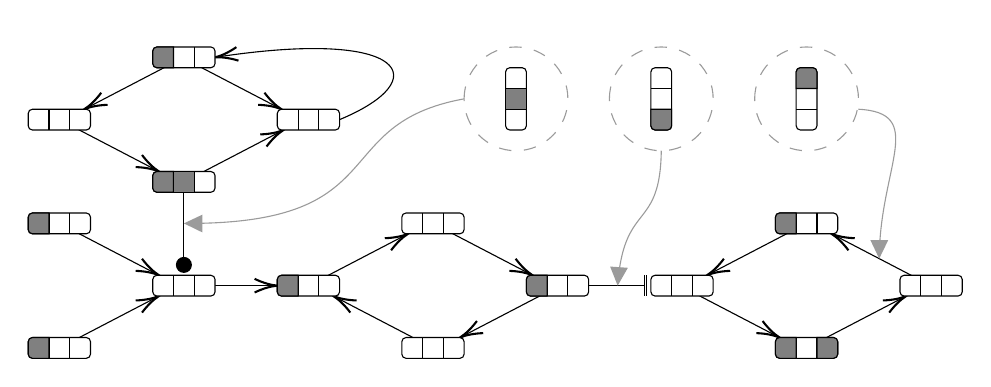
\begin{tikzpicture}[x=0.75pt,y=0.75pt,yscale=-1,xscale=1]
%uncomment if require: \path (0,300); %set diagram left start at 0, and has height of 300

%Straight Lines [id:da5482291659625731] 
\draw    (485,165) -- (438.77,140.92) ;
\draw [shift={(437,140)}, rotate = 387.51] [color={rgb, 255:red, 0; green, 0; blue, 0 }  ][line width=0.75]    (10.93,-3.29) .. controls (6.95,-1.4) and (3.31,-0.3) .. (0,0) .. controls (3.31,0.3) and (6.95,1.4) .. (10.93,3.29)   ;
%Straight Lines [id:da3558653268261338] 
\draw    (125,55) -- (78.77,79.08) ;
\draw [shift={(77,80)}, rotate = 332.49] [color={rgb, 255:red, 0; green, 0; blue, 0 }  ][line width=0.75]    (10.93,-3.29) .. controls (6.95,-1.4) and (3.31,-0.3) .. (0,0) .. controls (3.31,0.3) and (6.95,1.4) .. (10.93,3.29)   ;
%Straight Lines [id:da8145950972698188] 
\draw    (124,55) -- (170.23,79.08) ;
\draw [shift={(172,80)}, rotate = 207.51] [color={rgb, 255:red, 0; green, 0; blue, 0 }  ][line width=0.75]    (10.93,-3.29) .. controls (6.95,-1.4) and (3.31,-0.3) .. (0,0) .. controls (3.31,0.3) and (6.95,1.4) .. (10.93,3.29)   ;
%Curve Lines [id:da32133946156304494] 
\draw    (200,85) .. controls (246.69,65.62) and (232.66,40.97) .. (141.38,54.79) ;
\draw [shift={(140,55)}, rotate = 351.23] [color={rgb, 255:red, 0; green, 0; blue, 0 }  ][line width=0.75]    (10.93,-3.29) .. controls (6.95,-1.4) and (3.31,-0.3) .. (0,0) .. controls (3.31,0.3) and (6.95,1.4) .. (10.93,3.29)   ;
%Straight Lines [id:da041273036913917815] 
\draw    (65,85) -- (111.23,109.08) ;
\draw [shift={(113,110)}, rotate = 207.51] [color={rgb, 255:red, 0; green, 0; blue, 0 }  ][line width=0.75]    (10.93,-3.29) .. controls (6.95,-1.4) and (3.31,-0.3) .. (0,0) .. controls (3.31,0.3) and (6.95,1.4) .. (10.93,3.29)   ;
%Straight Lines [id:da8146569411368974] 
\draw    (125,115) -- (171.23,90.92) ;
\draw [shift={(173,90)}, rotate = 512.49] [color={rgb, 255:red, 0; green, 0; blue, 0 }  ][line width=0.75]    (10.93,-3.29) .. controls (6.95,-1.4) and (3.31,-0.3) .. (0,0) .. controls (3.31,0.3) and (6.95,1.4) .. (10.93,3.29)   ;
%Straight Lines [id:da3865035702712529] 
\draw    (125,115) -- (125,155) ;
\draw [shift={(125,155)}, rotate = 90] [color={rgb, 255:red, 0; green, 0; blue, 0 }  ][fill={rgb, 255:red, 0; green, 0; blue, 0 }  ][line width=0.75]      (0, 0) circle [x radius= 3.35, y radius= 3.35]   ;
%Straight Lines [id:da4717469304122126] 
\draw    (65,135) -- (111.23,159.08) ;
\draw [shift={(113,160)}, rotate = 207.51] [color={rgb, 255:red, 0; green, 0; blue, 0 }  ][line width=0.75]    (10.93,-3.29) .. controls (6.95,-1.4) and (3.31,-0.3) .. (0,0) .. controls (3.31,0.3) and (6.95,1.4) .. (10.93,3.29)   ;
%Straight Lines [id:da4798120333163296] 
\draw    (65,195) -- (111.23,170.92) ;
\draw [shift={(113,170)}, rotate = 512.49] [color={rgb, 255:red, 0; green, 0; blue, 0 }  ][line width=0.75]    (10.93,-3.29) .. controls (6.95,-1.4) and (3.31,-0.3) .. (0,0) .. controls (3.31,0.3) and (6.95,1.4) .. (10.93,3.29)   ;
%Straight Lines [id:da1936073846930204] 
\draw    (125,165) -- (168,165) ;
\draw [shift={(170,165)}, rotate = 180] [color={rgb, 255:red, 0; green, 0; blue, 0 }  ][line width=0.75]    (10.93,-3.29) .. controls (6.95,-1.4) and (3.31,-0.3) .. (0,0) .. controls (3.31,0.3) and (6.95,1.4) .. (10.93,3.29)   ;
%Straight Lines [id:da3160956298558728] 
\draw    (185,165) -- (231.23,140.92) ;
\draw [shift={(233,140)}, rotate = 512.49] [color={rgb, 255:red, 0; green, 0; blue, 0 }  ][line width=0.75]    (10.93,-3.29) .. controls (6.95,-1.4) and (3.31,-0.3) .. (0,0) .. controls (3.31,0.3) and (6.95,1.4) .. (10.93,3.29)   ;
%Straight Lines [id:da7125824842249591] 
\draw    (245,195) -- (198.77,170.92) ;
\draw [shift={(197,170)}, rotate = 387.51] [color={rgb, 255:red, 0; green, 0; blue, 0 }  ][line width=0.75]    (10.93,-3.29) .. controls (6.95,-1.4) and (3.31,-0.3) .. (0,0) .. controls (3.31,0.3) and (6.95,1.4) .. (10.93,3.29)   ;
%Straight Lines [id:da8854866739999274] 
\draw    (245,135) -- (291.23,159.08) ;
\draw [shift={(293,160)}, rotate = 207.51] [color={rgb, 255:red, 0; green, 0; blue, 0 }  ][line width=0.75]    (10.93,-3.29) .. controls (6.95,-1.4) and (3.31,-0.3) .. (0,0) .. controls (3.31,0.3) and (6.95,1.4) .. (10.93,3.29)   ;
%Straight Lines [id:da7803086702083197] 
\draw    (306,165) -- (259.77,189.08) ;
\draw [shift={(258,190)}, rotate = 332.49] [color={rgb, 255:red, 0; green, 0; blue, 0 }  ][line width=0.75]    (10.93,-3.29) .. controls (6.95,-1.4) and (3.31,-0.3) .. (0,0) .. controls (3.31,0.3) and (6.95,1.4) .. (10.93,3.29)   ;
%Straight Lines [id:da12899164332476598] 
\draw    (305,165) -- (347,165) ;
%Straight Lines [id:da7198750206752396] 
\draw    (425,135) -- (378.77,159.08) ;
\draw [shift={(377,160)}, rotate = 332.49] [color={rgb, 255:red, 0; green, 0; blue, 0 }  ][line width=0.75]    (10.93,-3.29) .. controls (6.95,-1.4) and (3.31,-0.3) .. (0,0) .. controls (3.31,0.3) and (6.95,1.4) .. (10.93,3.29)   ;
%Straight Lines [id:da9791465068682561] 
\draw    (364,165) -- (410.23,189.08) ;
\draw [shift={(412,190)}, rotate = 207.51] [color={rgb, 255:red, 0; green, 0; blue, 0 }  ][line width=0.75]    (10.93,-3.29) .. controls (6.95,-1.4) and (3.31,-0.3) .. (0,0) .. controls (3.31,0.3) and (6.95,1.4) .. (10.93,3.29)   ;
%Straight Lines [id:da6188188450953276] 
\draw    (425,195) -- (471.23,170.92) ;
\draw [shift={(473,170)}, rotate = 512.49] [color={rgb, 255:red, 0; green, 0; blue, 0 }  ][line width=0.75]    (10.93,-3.29) .. controls (6.95,-1.4) and (3.31,-0.3) .. (0,0) .. controls (3.31,0.3) and (6.95,1.4) .. (10.93,3.29)   ;
%Rounded Rect [id:dp8474040727349201] 
\draw  [fill={rgb, 255:red, 255; green, 255; blue, 255 }  ,fill opacity=1 ] (50,82) .. controls (50,80.9) and (50.9,80) .. (52,80) -- (78,80) .. controls (79.1,80) and (80,80.9) .. (80,82) -- (80,88) .. controls (80,89.1) and (79.1,90) .. (78,90) -- (52,90) .. controls (50.9,90) and (50,89.1) .. (50,88) -- cycle ;
%Straight Lines [id:da009868227811821173] 
\draw [fill={rgb, 255:red, 255; green, 255; blue, 255 }  ,fill opacity=1 ]   (60,80) -- (60,90) ;
%Straight Lines [id:da5531588010244222] 
\draw [fill={rgb, 255:red, 255; green, 255; blue, 255 }  ,fill opacity=1 ]   (70,80) -- (70,90) ;

%Rounded Rect [id:dp051842740859017855] 
\draw  [fill={rgb, 255:red, 255; green, 255; blue, 255 }  ,fill opacity=1 ] (110,52) .. controls (110,50.9) and (110.9,50) .. (112,50) -- (138,50) .. controls (139.1,50) and (140,50.9) .. (140,52) -- (140,58) .. controls (140,59.1) and (139.1,60) .. (138,60) -- (112,60) .. controls (110.9,60) and (110,59.1) .. (110,58) -- cycle ;
%Straight Lines [id:da9057225391135502] 
\draw [fill={rgb, 255:red, 255; green, 255; blue, 255 }  ,fill opacity=1 ]   (120,50) -- (120,60) ;
%Straight Lines [id:da6644491257645591] 
\draw [fill={rgb, 255:red, 255; green, 255; blue, 255 }  ,fill opacity=1 ]   (130,50) -- (130,60) ;

%Rounded Rect [id:dp6566561531995281] 
\draw  [fill={rgb, 255:red, 255; green, 255; blue, 255 }  ,fill opacity=1 ] (170,82) .. controls (170,80.9) and (170.9,80) .. (172,80) -- (198,80) .. controls (199.1,80) and (200,80.9) .. (200,82) -- (200,88) .. controls (200,89.1) and (199.1,90) .. (198,90) -- (172,90) .. controls (170.9,90) and (170,89.1) .. (170,88) -- cycle ;
%Straight Lines [id:da36189750423984623] 
\draw [fill={rgb, 255:red, 255; green, 255; blue, 255 }  ,fill opacity=1 ]   (180,80) -- (180,90) ;
%Straight Lines [id:da18569956496814277] 
\draw [fill={rgb, 255:red, 255; green, 255; blue, 255 }  ,fill opacity=1 ]   (190,80) -- (190,90) ;

%Rounded Rect [id:dp9774949153925689] 
\draw  [fill={rgb, 255:red, 255; green, 255; blue, 255 }  ,fill opacity=1 ] (110,112) .. controls (110,110.9) and (110.9,110) .. (112,110) -- (138,110) .. controls (139.1,110) and (140,110.9) .. (140,112) -- (140,118) .. controls (140,119.1) and (139.1,120) .. (138,120) -- (112,120) .. controls (110.9,120) and (110,119.1) .. (110,118) -- cycle ;
%Straight Lines [id:da8835613843611245] 
\draw [fill={rgb, 255:red, 255; green, 255; blue, 255 }  ,fill opacity=1 ]   (120,110) -- (120,120) ;
%Straight Lines [id:da046921024126330035] 
\draw [fill={rgb, 255:red, 255; green, 255; blue, 255 }  ,fill opacity=1 ]   (130,110) -- (130,120) ;

%Rounded Rect [id:dp9110792228160389] 
\draw  [fill={rgb, 255:red, 255; green, 255; blue, 255 }  ,fill opacity=1 ] (110,162) .. controls (110,160.9) and (110.9,160) .. (112,160) -- (138,160) .. controls (139.1,160) and (140,160.9) .. (140,162) -- (140,168) .. controls (140,169.1) and (139.1,170) .. (138,170) -- (112,170) .. controls (110.9,170) and (110,169.1) .. (110,168) -- cycle ;
%Straight Lines [id:da9579570207903243] 
\draw [fill={rgb, 255:red, 255; green, 255; blue, 255 }  ,fill opacity=1 ]   (120,160) -- (120,170) ;
%Straight Lines [id:da12487673944125555] 
\draw [fill={rgb, 255:red, 255; green, 255; blue, 255 }  ,fill opacity=1 ]   (130,160) -- (130,170) ;

%Rounded Rect [id:dp6019071628472181] 
\draw  [fill={rgb, 255:red, 255; green, 255; blue, 255 }  ,fill opacity=1 ] (50,132) .. controls (50,130.9) and (50.9,130) .. (52,130) -- (78,130) .. controls (79.1,130) and (80,130.9) .. (80,132) -- (80,138) .. controls (80,139.1) and (79.1,140) .. (78,140) -- (52,140) .. controls (50.9,140) and (50,139.1) .. (50,138) -- cycle ;
%Straight Lines [id:da07709686395947624] 
\draw [fill={rgb, 255:red, 255; green, 255; blue, 255 }  ,fill opacity=1 ]   (60,130) -- (60,140) ;
%Straight Lines [id:da4386719436852351] 
\draw [fill={rgb, 255:red, 255; green, 255; blue, 255 }  ,fill opacity=1 ]   (70,130) -- (70,140) ;

%Rounded Rect [id:dp7005531294638312] 
\draw  [fill={rgb, 255:red, 255; green, 255; blue, 255 }  ,fill opacity=1 ] (50,192) .. controls (50,190.9) and (50.9,190) .. (52,190) -- (78,190) .. controls (79.1,190) and (80,190.9) .. (80,192) -- (80,198) .. controls (80,199.1) and (79.1,200) .. (78,200) -- (52,200) .. controls (50.9,200) and (50,199.1) .. (50,198) -- cycle ;
%Straight Lines [id:da5611530770018562] 
\draw [fill={rgb, 255:red, 255; green, 255; blue, 255 }  ,fill opacity=1 ]   (60,190) -- (60,200) ;
%Straight Lines [id:da017232921254101363] 
\draw [fill={rgb, 255:red, 255; green, 255; blue, 255 }  ,fill opacity=1 ]   (70,190) -- (70,200) ;

%Rounded Rect [id:dp4827173759682435] 
\draw  [fill={rgb, 255:red, 255; green, 255; blue, 255 }  ,fill opacity=1 ] (170,162) .. controls (170,160.9) and (170.9,160) .. (172,160) -- (198,160) .. controls (199.1,160) and (200,160.9) .. (200,162) -- (200,168) .. controls (200,169.1) and (199.1,170) .. (198,170) -- (172,170) .. controls (170.9,170) and (170,169.1) .. (170,168) -- cycle ;
%Straight Lines [id:da9642172775022364] 
\draw [fill={rgb, 255:red, 255; green, 255; blue, 255 }  ,fill opacity=1 ]   (180,160) -- (180,170) ;
%Straight Lines [id:da7596136700374254] 
\draw [fill={rgb, 255:red, 255; green, 255; blue, 255 }  ,fill opacity=1 ]   (190,160) -- (190,170) ;

%Rounded Rect [id:dp6674528307093845] 
\draw  [fill={rgb, 255:red, 255; green, 255; blue, 255 }  ,fill opacity=1 ] (230,132) .. controls (230,130.9) and (230.9,130) .. (232,130) -- (258,130) .. controls (259.1,130) and (260,130.9) .. (260,132) -- (260,138) .. controls (260,139.1) and (259.1,140) .. (258,140) -- (232,140) .. controls (230.9,140) and (230,139.1) .. (230,138) -- cycle ;
%Straight Lines [id:da2821204278394096] 
\draw [fill={rgb, 255:red, 255; green, 255; blue, 255 }  ,fill opacity=1 ]   (240,130) -- (240,140) ;
%Straight Lines [id:da12264275434933958] 
\draw [fill={rgb, 255:red, 255; green, 255; blue, 255 }  ,fill opacity=1 ]   (250,130) -- (250,140) ;

%Rounded Rect [id:dp35957703897594406] 
\draw  [fill={rgb, 255:red, 255; green, 255; blue, 255 }  ,fill opacity=1 ] (290,162) .. controls (290,160.9) and (290.9,160) .. (292,160) -- (318,160) .. controls (319.1,160) and (320,160.9) .. (320,162) -- (320,168) .. controls (320,169.1) and (319.1,170) .. (318,170) -- (292,170) .. controls (290.9,170) and (290,169.1) .. (290,168) -- cycle ;
%Straight Lines [id:da523669754182625] 
\draw [fill={rgb, 255:red, 255; green, 255; blue, 255 }  ,fill opacity=1 ]   (300,160) -- (300,170) ;
%Straight Lines [id:da3829127214939474] 
\draw [fill={rgb, 255:red, 255; green, 255; blue, 255 }  ,fill opacity=1 ]   (310,160) -- (310,170) ;

%Rounded Rect [id:dp42701231482854474] 
\draw  [fill={rgb, 255:red, 255; green, 255; blue, 255 }  ,fill opacity=1 ] (230,192) .. controls (230,190.9) and (230.9,190) .. (232,190) -- (258,190) .. controls (259.1,190) and (260,190.9) .. (260,192) -- (260,198) .. controls (260,199.1) and (259.1,200) .. (258,200) -- (232,200) .. controls (230.9,200) and (230,199.1) .. (230,198) -- cycle ;
%Straight Lines [id:da42410503561121105] 
\draw [fill={rgb, 255:red, 255; green, 255; blue, 255 }  ,fill opacity=1 ]   (240,190) -- (240,200) ;
%Straight Lines [id:da3684047905504595] 
\draw [fill={rgb, 255:red, 255; green, 255; blue, 255 }  ,fill opacity=1 ]   (250,190) -- (250,200) ;

%Rounded Rect [id:dp11445404510516877] 
\draw  [fill={rgb, 255:red, 255; green, 255; blue, 255 }  ,fill opacity=1 ] (350,162) .. controls (350,160.9) and (350.9,160) .. (352,160) -- (378,160) .. controls (379.1,160) and (380,160.9) .. (380,162) -- (380,168) .. controls (380,169.1) and (379.1,170) .. (378,170) -- (352,170) .. controls (350.9,170) and (350,169.1) .. (350,168) -- cycle ;
%Straight Lines [id:da43972531825515127] 
\draw [fill={rgb, 255:red, 255; green, 255; blue, 255 }  ,fill opacity=1 ]   (360,160) -- (360,170) ;
%Straight Lines [id:da5041547924292167] 
\draw [fill={rgb, 255:red, 255; green, 255; blue, 255 }  ,fill opacity=1 ]   (370,160) -- (370,170) ;

%Rounded Rect [id:dp4489618141059677] 
\draw  [fill={rgb, 255:red, 255; green, 255; blue, 255 }  ,fill opacity=1 ] (410,132) .. controls (410,130.9) and (410.9,130) .. (412,130) -- (438,130) .. controls (439.1,130) and (440,130.9) .. (440,132) -- (440,138) .. controls (440,139.1) and (439.1,140) .. (438,140) -- (412,140) .. controls (410.9,140) and (410,139.1) .. (410,138) -- cycle ;
%Straight Lines [id:da13613343685552803] 
\draw [fill={rgb, 255:red, 255; green, 255; blue, 255 }  ,fill opacity=1 ]   (420,130) -- (420,140) ;
%Straight Lines [id:da1649141879778826] 
\draw [fill={rgb, 255:red, 255; green, 255; blue, 255 }  ,fill opacity=1 ]   (430,130) -- (430,140) ;

%Rounded Rect [id:dp085382714873663] 
\draw  [fill={rgb, 255:red, 255; green, 255; blue, 255 }  ,fill opacity=1 ] (470,162) .. controls (470,160.9) and (470.9,160) .. (472,160) -- (498,160) .. controls (499.1,160) and (500,160.9) .. (500,162) -- (500,168) .. controls (500,169.1) and (499.1,170) .. (498,170) -- (472,170) .. controls (470.9,170) and (470,169.1) .. (470,168) -- cycle ;
%Straight Lines [id:da7027806909135705] 
\draw [fill={rgb, 255:red, 255; green, 255; blue, 255 }  ,fill opacity=1 ]   (480,160) -- (480,170) ;
%Straight Lines [id:da6677143633674809] 
\draw [fill={rgb, 255:red, 255; green, 255; blue, 255 }  ,fill opacity=1 ]   (490,160) -- (490,170) ;

%Rounded Rect [id:dp23601106803709837] 
\draw  [fill={rgb, 255:red, 255; green, 255; blue, 255 }  ,fill opacity=1 ] (410,192) .. controls (410,190.9) and (410.9,190) .. (412,190) -- (438,190) .. controls (439.1,190) and (440,190.9) .. (440,192) -- (440,198) .. controls (440,199.1) and (439.1,200) .. (438,200) -- (412,200) .. controls (410.9,200) and (410,199.1) .. (410,198) -- cycle ;
%Straight Lines [id:da7303797329340842] 
\draw [fill={rgb, 255:red, 255; green, 255; blue, 255 }  ,fill opacity=1 ]   (420,190) -- (420,200) ;
%Straight Lines [id:da7412443437267568] 
\draw [fill={rgb, 255:red, 255; green, 255; blue, 255 }  ,fill opacity=1 ]   (430,190) -- (430,200) ;

%Straight Lines [id:da011003964046166548] 
\draw    (347,160) -- (347,170) ;
%Straight Lines [id:da9806624892870546] 
\draw    (348,160) -- (348,170) ;

%Rounded Same Side Corner Rect [id:dp3768094591748803] 
\draw  [fill={rgb, 255:red, 128; green, 128; blue, 128 }  ,fill opacity=1 ] (112,120) .. controls (110.9,120) and (110,119.1) .. (110,118) -- (110,112) .. controls (110,110.9) and (110.9,110) .. (112,110) -- (120,110) .. controls (120,110) and (120,110) .. (120,110) -- (120,120) .. controls (120,120) and (120,120) .. (120,120) -- cycle ;
%Rounded Same Side Corner Rect [id:dp9234675571457911] 
\draw  [fill={rgb, 255:red, 128; green, 128; blue, 128 }  ,fill opacity=1 ] (52,140) .. controls (50.9,140) and (50,139.1) .. (50,138) -- (50,132) .. controls (50,130.9) and (50.9,130) .. (52,130) -- (60,130) .. controls (60,130) and (60,130) .. (60,130) -- (60,140) .. controls (60,140) and (60,140) .. (60,140) -- cycle ;
%Rounded Same Side Corner Rect [id:dp5054471322165766] 
\draw  [fill={rgb, 255:red, 128; green, 128; blue, 128 }  ,fill opacity=1 ] (52,200) .. controls (50.9,200) and (50,199.1) .. (50,198) -- (50,192) .. controls (50,190.9) and (50.9,190) .. (52,190) -- (60,190) .. controls (60,190) and (60,190) .. (60,190) -- (60,200) .. controls (60,200) and (60,200) .. (60,200) -- cycle ;
%Rounded Same Side Corner Rect [id:dp3931764941128213] 
\draw  [fill={rgb, 255:red, 128; green, 128; blue, 128 }  ,fill opacity=1 ] (112,60) .. controls (110.9,60) and (110,59.1) .. (110,58) -- (110,52) .. controls (110,50.9) and (110.9,50) .. (112,50) -- (120,50) .. controls (120,50) and (120,50) .. (120,50) -- (120,60) .. controls (120,60) and (120,60) .. (120,60) -- cycle ;
%Rounded Same Side Corner Rect [id:dp2835639273199655] 
\draw  [fill={rgb, 255:red, 128; green, 128; blue, 128 }  ,fill opacity=1 ] (172,170) .. controls (170.9,170) and (170,169.1) .. (170,168) -- (170,162) .. controls (170,160.9) and (170.9,160) .. (172,160) -- (180,160) .. controls (180,160) and (180,160) .. (180,160) -- (180,170) .. controls (180,170) and (180,170) .. (180,170) -- cycle ;
%Rounded Same Side Corner Rect [id:dp9984840474478471] 
\draw  [fill={rgb, 255:red, 128; green, 128; blue, 128 }  ,fill opacity=1 ] (292,170) .. controls (290.9,170) and (290,169.1) .. (290,168) -- (290,162) .. controls (290,160.9) and (290.9,160) .. (292,160) -- (300,160) .. controls (300,160) and (300,160) .. (300,160) -- (300,170) .. controls (300,170) and (300,170) .. (300,170) -- cycle ;
%Rounded Same Side Corner Rect [id:dp9874301673779244] 
\draw  [fill={rgb, 255:red, 128; green, 128; blue, 128 }  ,fill opacity=1 ] (412,140) .. controls (410.9,140) and (410,139.1) .. (410,138) -- (410,132) .. controls (410,130.9) and (410.9,130) .. (412,130) -- (420,130) .. controls (420,130) and (420,130) .. (420,130) -- (420,140) .. controls (420,140) and (420,140) .. (420,140) -- cycle ;
%Rounded Same Side Corner Rect [id:dp17981279327281907] 
\draw  [fill={rgb, 255:red, 128; green, 128; blue, 128 }  ,fill opacity=1 ] (412,200) .. controls (410.9,200) and (410,199.1) .. (410,198) -- (410,192) .. controls (410,190.9) and (410.9,190) .. (412,190) -- (420,190) .. controls (420,190) and (420,190) .. (420,190) -- (420,200) .. controls (420,200) and (420,200) .. (420,200) -- cycle ;
%Shape: Rectangle [id:dp9896265723760629] 
\draw  [fill={rgb, 255:red, 128; green, 128; blue, 128 }  ,fill opacity=1 ] (120,110) -- (130,110) -- (130,120) -- (120,120) -- cycle ;
%Rounded Same Side Corner Rect [id:dp6704577445807436] 
\draw  [fill={rgb, 255:red, 128; green, 128; blue, 128 }  ,fill opacity=1 ] (438,190) .. controls (439.1,190) and (440,190.9) .. (440,192) -- (440,198) .. controls (440,199.1) and (439.1,200) .. (438,200) -- (430,200) .. controls (430,200) and (430,200) .. (430,200) -- (430,190) .. controls (430,190) and (430,190) .. (430,190) -- cycle ;
%Rounded Rect [id:dp11409130649511323] 
\draw  [fill={rgb, 255:red, 255; green, 255; blue, 255 }  ,fill opacity=1 ] (288,60) .. controls (289.1,60) and (290,60.9) .. (290,62) -- (290,88) .. controls (290,89.1) and (289.1,90) .. (288,90) -- (282,90) .. controls (280.9,90) and (280,89.1) .. (280,88) -- (280,62) .. controls (280,60.9) and (280.9,60) .. (282,60) -- cycle ;
%Straight Lines [id:da8566613339394187] 
\draw [fill={rgb, 255:red, 255; green, 255; blue, 255 }  ,fill opacity=1 ]   (290,70) -- (280,70) ;
%Straight Lines [id:da6431189043654337] 
\draw [fill={rgb, 255:red, 255; green, 255; blue, 255 }  ,fill opacity=1 ]   (290,80) -- (280,80) ;

%Curve Lines [id:da9261031951036094] 
\draw [color={rgb, 255:red, 155; green, 155; blue, 155 }  ,draw opacity=1 ]   (260,75) .. controls (193.53,87.09) and (227.36,135.17) .. (126.53,135.01) ;
\draw [shift={(125,135)}, rotate = 360.36] [fill={rgb, 255:red, 155; green, 155; blue, 155 }  ,fill opacity=1 ][line width=0.08]  [draw opacity=0] (8.93,-4.29) -- (0,0) -- (8.93,4.29) -- cycle    ;
%Shape: Circle [id:dp642495337158681] 
\draw  [color={rgb, 255:red, 155; green, 155; blue, 155 }  ,draw opacity=1 ][dash pattern={on 4.5pt off 4.5pt}] (260,75) .. controls (260,61.19) and (271.19,50) .. (285,50) .. controls (298.81,50) and (310,61.19) .. (310,75) .. controls (310,88.81) and (298.81,100) .. (285,100) .. controls (271.19,100) and (260,88.81) .. (260,75) -- cycle ;
%Rounded Rect [id:dp7279380411207359] 
\draw  [fill={rgb, 255:red, 255; green, 255; blue, 255 }  ,fill opacity=1 ] (358,60) .. controls (359.1,60) and (360,60.9) .. (360,62) -- (360,88) .. controls (360,89.1) and (359.1,90) .. (358,90) -- (352,90) .. controls (350.9,90) and (350,89.1) .. (350,88) -- (350,62) .. controls (350,60.9) and (350.9,60) .. (352,60) -- cycle ;
%Straight Lines [id:da643323388211388] 
\draw [fill={rgb, 255:red, 255; green, 255; blue, 255 }  ,fill opacity=1 ]   (360,70) -- (350,70) ;
%Straight Lines [id:da9235014852609569] 
\draw [fill={rgb, 255:red, 255; green, 255; blue, 255 }  ,fill opacity=1 ]   (360,80) -- (350,80) ;

%Shape: Circle [id:dp14795654137945813] 
\draw  [color={rgb, 255:red, 155; green, 155; blue, 155 }  ,draw opacity=1 ][dash pattern={on 4.5pt off 4.5pt}] (330,75) .. controls (330,61.19) and (341.19,50) .. (355,50) .. controls (368.81,50) and (380,61.19) .. (380,75) .. controls (380,88.81) and (368.81,100) .. (355,100) .. controls (341.19,100) and (330,88.81) .. (330,75) -- cycle ;
%Curve Lines [id:da714596365164035] 
\draw [color={rgb, 255:red, 155; green, 155; blue, 155 }  ,draw opacity=1 ]   (355,100) .. controls (354.49,138.16) and (337.75,124.67) .. (334.24,162.02) ;
\draw [shift={(334,165)}, rotate = 274.01] [fill={rgb, 255:red, 155; green, 155; blue, 155 }  ,fill opacity=1 ][line width=0.08]  [draw opacity=0] (8.93,-4.29) -- (0,0) -- (8.93,4.29) -- cycle    ;
%Rounded Rect [id:dp7787064930154233] 
\draw  [fill={rgb, 255:red, 255; green, 255; blue, 255 }  ,fill opacity=1 ] (428,60) .. controls (429.1,60) and (430,60.9) .. (430,62) -- (430,88) .. controls (430,89.1) and (429.1,90) .. (428,90) -- (422,90) .. controls (420.9,90) and (420,89.1) .. (420,88) -- (420,62) .. controls (420,60.9) and (420.9,60) .. (422,60) -- cycle ;
%Straight Lines [id:da6888394852686113] 
\draw [fill={rgb, 255:red, 255; green, 255; blue, 255 }  ,fill opacity=1 ]   (430,70) -- (420,70) ;
%Straight Lines [id:da5007706839755712] 
\draw [fill={rgb, 255:red, 255; green, 255; blue, 255 }  ,fill opacity=1 ]   (430,80) -- (420,80) ;

%Shape: Circle [id:dp9185294933885089] 
\draw  [color={rgb, 255:red, 155; green, 155; blue, 155 }  ,draw opacity=1 ][dash pattern={on 4.5pt off 4.5pt}] (400,75) .. controls (400,61.19) and (411.19,50) .. (425,50) .. controls (438.81,50) and (450,61.19) .. (450,75) .. controls (450,88.81) and (438.81,100) .. (425,100) .. controls (411.19,100) and (400,88.81) .. (400,75) -- cycle ;
%Curve Lines [id:da2587793508415681] 
\draw [color={rgb, 255:red, 155; green, 155; blue, 155 }  ,draw opacity=1 ]   (450,80) .. controls (482.54,81.72) and (461.1,106.72) .. (460.04,149.37) ;
\draw [shift={(460,152)}, rotate = 270.26] [fill={rgb, 255:red, 155; green, 155; blue, 155 }  ,fill opacity=1 ][line width=0.08]  [draw opacity=0] (8.93,-4.29) -- (0,0) -- (8.93,4.29) -- cycle    ;
%Rounded Same Side Corner Rect [id:dp9448859813691737] 
\draw  [fill={rgb, 255:red, 128; green, 128; blue, 128 }  ,fill opacity=1 ] (360,88) .. controls (360,89.1) and (359.1,90) .. (358,90) -- (352,90) .. controls (350.9,90) and (350,89.1) .. (350,88) -- (350,80) .. controls (350,80) and (350,80) .. (350,80) -- (360,80) .. controls (360,80) and (360,80) .. (360,80) -- cycle ;
%Rounded Same Side Corner Rect [id:dp22917183902440952] 
\draw  [fill={rgb, 255:red, 128; green, 128; blue, 128 }  ,fill opacity=1 ] (420,62) .. controls (420,60.9) and (420.9,60) .. (422,60) -- (428,60) .. controls (429.1,60) and (430,60.9) .. (430,62) -- (430,70) .. controls (430,70) and (430,70) .. (430,70) -- (420,70) .. controls (420,70) and (420,70) .. (420,70) -- cycle ;
%Shape: Rectangle [id:dp6259213163981312] 
\draw  [fill={rgb, 255:red, 128; green, 128; blue, 128 }  ,fill opacity=1 ] (280,70) -- (290,70) -- (290,80) -- (280,80) -- cycle ;




\end{tikzpicture}}
    \caption{A representation of the node and edge feature vectors of the induced subgraph shown in Figure \ref{subfig:subgraph3}. Each node is represented as a 3-dimensional binary vector, where 1 is indicated with dark grey and 0 with white. To avoid visual cluttering, we only show one example of edge feature vector per edge type (the column vectors inside the dashed circles).}
    \label{fig:pathway-graph-features}
\end{figure*}

\section{Experiments}\label{sec:pathway-experiments}
In this section, we provide all the necessary details concerning our experimental procedures. In particular, we describe the architecture of the \gls{dgn} in detail, and discuss the assessment protocol by which we evaluated the proposed model on the predictive task.

The proposed \gls{dgn} architecture for robustness prediction, shown at a high level in Figure \ref{fig:architecture}, consists in a series of $L$ graph convolutional layers, followed by a node readout that aggregates the hidden states at each layer into node representations by concatenation, a graph readout that aggregates the node representations into a graph representation, and a downstream \gls{mlp} classifier which uses the graph representation to compute a probability of whether the graph is robust or not.
\begin{figure*}[h!]
    \centering
    \resizebox{.95\textwidth}{!}{

\tikzset{every picture/.style={line width=0.75pt}} %set default line width to 0.75pt

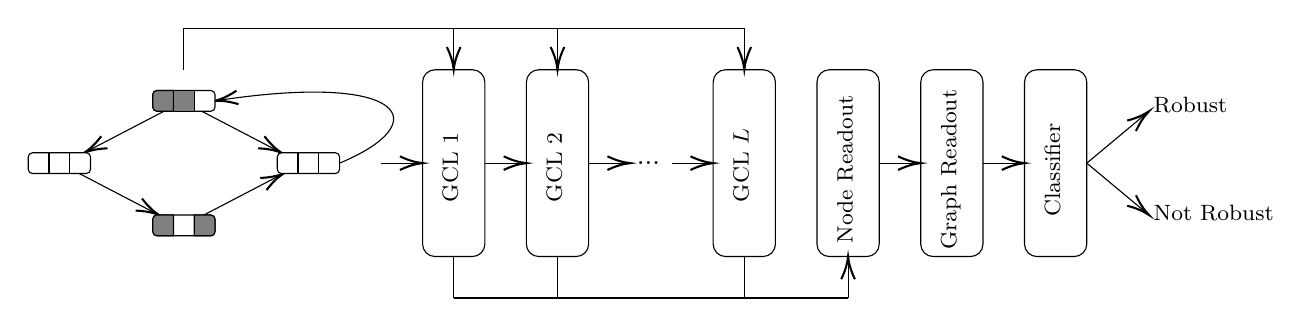
\begin{tikzpicture}[x=0.75pt,y=0.75pt,yscale=-1,xscale=1]
%uncomment if require: \path (0,222); %set diagram left start at 0, and has height of 222

%Straight Lines [id:da10249777348922673]
\draw    (105,55) -- (58.77,79.08) ;
\draw [shift={(57,80)}, rotate = 332.49] [color={rgb, 255:red, 0; green, 0; blue, 0 }  ][line width=0.75]    (10.93,-3.29) .. controls (6.95,-1.4) and (3.31,-0.3) .. (0,0) .. controls (3.31,0.3) and (6.95,1.4) .. (10.93,3.29)   ;
%Straight Lines [id:da8543699837088969]
\draw    (104,55) -- (150.23,79.08) ;
\draw [shift={(152,80)}, rotate = 207.51] [color={rgb, 255:red, 0; green, 0; blue, 0 }  ][line width=0.75]    (10.93,-3.29) .. controls (6.95,-1.4) and (3.31,-0.3) .. (0,0) .. controls (3.31,0.3) and (6.95,1.4) .. (10.93,3.29)   ;
%Curve Lines [id:da718018348959689]
\draw    (180,85) .. controls (226.69,65.62) and (212.66,40.97) .. (121.38,54.79) ;
\draw [shift={(120,55)}, rotate = 351.23] [color={rgb, 255:red, 0; green, 0; blue, 0 }  ][line width=0.75]    (10.93,-3.29) .. controls (6.95,-1.4) and (3.31,-0.3) .. (0,0) .. controls (3.31,0.3) and (6.95,1.4) .. (10.93,3.29)   ;
%Straight Lines [id:da40161395618619355]
\draw    (45,85) -- (91.23,109.08) ;
\draw [shift={(93,110)}, rotate = 207.51] [color={rgb, 255:red, 0; green, 0; blue, 0 }  ][line width=0.75]    (10.93,-3.29) .. controls (6.95,-1.4) and (3.31,-0.3) .. (0,0) .. controls (3.31,0.3) and (6.95,1.4) .. (10.93,3.29)   ;
%Straight Lines [id:da9404547371703709]
\draw    (105,115) -- (151.23,90.92) ;
\draw [shift={(153,90)}, rotate = 512.49] [color={rgb, 255:red, 0; green, 0; blue, 0 }  ][line width=0.75]    (10.93,-3.29) .. controls (6.95,-1.4) and (3.31,-0.3) .. (0,0) .. controls (3.31,0.3) and (6.95,1.4) .. (10.93,3.29)   ;
%Rounded Rect [id:dp8918717737625625]
\draw  [fill={rgb, 255:red, 255; green, 255; blue, 255 }  ,fill opacity=1 ] (30,82) .. controls (30,80.9) and (30.9,80) .. (32,80) -- (58,80) .. controls (59.1,80) and (60,80.9) .. (60,82) -- (60,88) .. controls (60,89.1) and (59.1,90) .. (58,90) -- (32,90) .. controls (30.9,90) and (30,89.1) .. (30,88) -- cycle ;
%Straight Lines [id:da2840220975641643]
\draw [fill={rgb, 255:red, 255; green, 255; blue, 255 }  ,fill opacity=1 ]   (40,80) -- (40,90) ;
%Straight Lines [id:da9928129104895596]
\draw [fill={rgb, 255:red, 255; green, 255; blue, 255 }  ,fill opacity=1 ]   (50,80) -- (50,90) ;

%Rounded Rect [id:dp657055048085913]
\draw  [fill={rgb, 255:red, 255; green, 255; blue, 255 }  ,fill opacity=1 ] (90,52) .. controls (90,50.9) and (90.9,50) .. (92,50) -- (118,50) .. controls (119.1,50) and (120,50.9) .. (120,52) -- (120,58) .. controls (120,59.1) and (119.1,60) .. (118,60) -- (92,60) .. controls (90.9,60) and (90,59.1) .. (90,58) -- cycle ;
%Straight Lines [id:da38800902985878216]
\draw [fill={rgb, 255:red, 255; green, 255; blue, 255 }  ,fill opacity=1 ]   (100,50) -- (100,60) ;
%Straight Lines [id:da35157806490529486]
\draw [fill={rgb, 255:red, 255; green, 255; blue, 255 }  ,fill opacity=1 ]   (110,50) -- (110,60) ;

%Rounded Rect [id:dp8042816045609678]
\draw  [fill={rgb, 255:red, 255; green, 255; blue, 255 }  ,fill opacity=1 ] (150,82) .. controls (150,80.9) and (150.9,80) .. (152,80) -- (178,80) .. controls (179.1,80) and (180,80.9) .. (180,82) -- (180,88) .. controls (180,89.1) and (179.1,90) .. (178,90) -- (152,90) .. controls (150.9,90) and (150,89.1) .. (150,88) -- cycle ;
%Straight Lines [id:da6303967094544072]
\draw [fill={rgb, 255:red, 255; green, 255; blue, 255 }  ,fill opacity=1 ]   (160,80) -- (160,90) ;
%Straight Lines [id:da38699794541515686]
\draw [fill={rgb, 255:red, 255; green, 255; blue, 255 }  ,fill opacity=1 ]   (170,80) -- (170,90) ;

%Rounded Rect [id:dp30617610846254983]
\draw  [fill={rgb, 255:red, 255; green, 255; blue, 255 }  ,fill opacity=1 ] (90,112) .. controls (90,110.9) and (90.9,110) .. (92,110) -- (118,110) .. controls (119.1,110) and (120,110.9) .. (120,112) -- (120,118) .. controls (120,119.1) and (119.1,120) .. (118,120) -- (92,120) .. controls (90.9,120) and (90,119.1) .. (90,118) -- cycle ;
%Straight Lines [id:da5849892704416262]
\draw [fill={rgb, 255:red, 255; green, 255; blue, 255 }  ,fill opacity=1 ]   (100,110) -- (100,120) ;
%Straight Lines [id:da5154765063607318]
\draw [fill={rgb, 255:red, 255; green, 255; blue, 255 }  ,fill opacity=1 ]   (110,110) -- (110,120) ;

%Rounded Same Side Corner Rect [id:dp16054859719249248]
\draw  [fill={rgb, 255:red, 128; green, 128; blue, 128 }  ,fill opacity=1 ] (92,120) .. controls (90.9,120) and (90,119.1) .. (90,118) -- (90,112) .. controls (90,110.9) and (90.9,110) .. (92,110) -- (100,110) .. controls (100,110) and (100,110) .. (100,110) -- (100,120) .. controls (100,120) and (100,120) .. (100,120) -- cycle ;
%Rounded Same Side Corner Rect [id:dp4777662533474829]
\draw  [fill={rgb, 255:red, 128; green, 128; blue, 128 }  ,fill opacity=1 ] (92,60) .. controls (90.9,60) and (90,59.1) .. (90,58) -- (90,52) .. controls (90,50.9) and (90.9,50) .. (92,50) -- (100,50) .. controls (100,50) and (100,50) .. (100,50) -- (100,60) .. controls (100,60) and (100,60) .. (100,60) -- cycle ;
%Rounded Rect [id:dp2612266462776953]
\draw   (220,46) .. controls (220,42.69) and (222.69,40) .. (226,40) -- (244,40) .. controls (247.31,40) and (250,42.69) .. (250,46) -- (250,124) .. controls (250,127.31) and (247.31,130) .. (244,130) -- (226,130) .. controls (222.69,130) and (220,127.31) .. (220,124) -- cycle ;
%Rounded Rect [id:dp6049233789003581]
\draw   (270,46) .. controls (270,42.69) and (272.69,40) .. (276,40) -- (294,40) .. controls (297.31,40) and (300,42.69) .. (300,46) -- (300,124) .. controls (300,127.31) and (297.31,130) .. (294,130) -- (276,130) .. controls (272.69,130) and (270,127.31) .. (270,124) -- cycle ;
%Rounded Rect [id:dp9219708545047745]
\draw   (360,46) .. controls (360,42.69) and (362.69,40) .. (366,40) -- (384,40) .. controls (387.31,40) and (390,42.69) .. (390,46) -- (390,124) .. controls (390,127.31) and (387.31,130) .. (384,130) -- (366,130) .. controls (362.69,130) and (360,127.31) .. (360,124) -- cycle ;
%Rounded Rect [id:dp06877784323777258]
\draw   (410,46) .. controls (410,42.69) and (412.69,40) .. (416,40) -- (434,40) .. controls (437.31,40) and (440,42.69) .. (440,46) -- (440,124) .. controls (440,127.31) and (437.31,130) .. (434,130) -- (416,130) .. controls (412.69,130) and (410,127.31) .. (410,124) -- cycle ;
%Straight Lines [id:da3242474162330802]
\draw    (105,20) -- (105,40) ;
%Straight Lines [id:da3678823594719134]
\draw    (105,20) -- (375,20) ;
%Straight Lines [id:da48488761692333315]
\draw    (200,85) -- (218,85) ;
\draw [shift={(220,85)}, rotate = 180] [color={rgb, 255:red, 0; green, 0; blue, 0 }  ][line width=0.75]    (10.93,-3.29) .. controls (6.95,-1.4) and (3.31,-0.3) .. (0,0) .. controls (3.31,0.3) and (6.95,1.4) .. (10.93,3.29)   ;
%Straight Lines [id:da7353824116605796]
\draw    (250,85) -- (268,85) ;
\draw [shift={(270,85)}, rotate = 180] [color={rgb, 255:red, 0; green, 0; blue, 0 }  ][line width=0.75]    (10.93,-3.29) .. controls (6.95,-1.4) and (3.31,-0.3) .. (0,0) .. controls (3.31,0.3) and (6.95,1.4) .. (10.93,3.29)   ;
%Straight Lines [id:da621667250955845]
\draw    (300,85) -- (318,85) ;
\draw [shift={(320,85)}, rotate = 180] [color={rgb, 255:red, 0; green, 0; blue, 0 }  ][line width=0.75]    (10.93,-3.29) .. controls (6.95,-1.4) and (3.31,-0.3) .. (0,0) .. controls (3.31,0.3) and (6.95,1.4) .. (10.93,3.29)   ;
%Straight Lines [id:da0389620564663371]
\draw    (340,85) -- (358,85) ;
\draw [shift={(360,85)}, rotate = 180] [color={rgb, 255:red, 0; green, 0; blue, 0 }  ][line width=0.75]    (10.93,-3.29) .. controls (6.95,-1.4) and (3.31,-0.3) .. (0,0) .. controls (3.31,0.3) and (6.95,1.4) .. (10.93,3.29)   ;
%Straight Lines [id:da49854406681907104]
\draw    (235,20) -- (235,38) ;
\draw [shift={(235,40)}, rotate = 270] [color={rgb, 255:red, 0; green, 0; blue, 0 }  ][line width=0.75]    (10.93,-3.29) .. controls (6.95,-1.4) and (3.31,-0.3) .. (0,0) .. controls (3.31,0.3) and (6.95,1.4) .. (10.93,3.29)   ;
%Straight Lines [id:da3320143976606864]
\draw    (285,20) -- (285,38) ;
\draw [shift={(285,40)}, rotate = 270] [color={rgb, 255:red, 0; green, 0; blue, 0 }  ][line width=0.75]    (10.93,-3.29) .. controls (6.95,-1.4) and (3.31,-0.3) .. (0,0) .. controls (3.31,0.3) and (6.95,1.4) .. (10.93,3.29)   ;
%Straight Lines [id:da0031583922795141994]
\draw    (375,20) -- (375,38) ;
\draw [shift={(375,40)}, rotate = 270] [color={rgb, 255:red, 0; green, 0; blue, 0 }  ][line width=0.75]    (10.93,-3.29) .. controls (6.95,-1.4) and (3.31,-0.3) .. (0,0) .. controls (3.31,0.3) and (6.95,1.4) .. (10.93,3.29)   ;
%Straight Lines [id:da6752204950269405]
\draw    (440,85) -- (458,85) ;
\draw [shift={(460,85)}, rotate = 180] [color={rgb, 255:red, 0; green, 0; blue, 0 }  ][line width=0.75]    (10.93,-3.29) .. controls (6.95,-1.4) and (3.31,-0.3) .. (0,0) .. controls (3.31,0.3) and (6.95,1.4) .. (10.93,3.29)   ;
%Rounded Rect [id:dp17194220548550754]
\draw   (460,46) .. controls (460,42.69) and (462.69,40) .. (466,40) -- (484,40) .. controls (487.31,40) and (490,42.69) .. (490,46) -- (490,124) .. controls (490,127.31) and (487.31,130) .. (484,130) -- (466,130) .. controls (462.69,130) and (460,127.31) .. (460,124) -- cycle ;
%Straight Lines [id:da6487892442997589]
\draw    (490,85) -- (508,85) ;
\draw [shift={(510,85)}, rotate = 180] [color={rgb, 255:red, 0; green, 0; blue, 0 }  ][line width=0.75]    (10.93,-3.29) .. controls (6.95,-1.4) and (3.31,-0.3) .. (0,0) .. controls (3.31,0.3) and (6.95,1.4) .. (10.93,3.29)   ;
%Straight Lines [id:da05300848730559804]
\draw    (235,130) -- (235,150) ;
%Straight Lines [id:da3909014389203407]
\draw    (285,130) -- (285,150) ;
%Straight Lines [id:da6126666581003337]
\draw    (375,130) -- (375,150) ;
%Straight Lines [id:da02140734221954288]
\draw    (425,150) -- (425,132) ;
\draw [shift={(425,130)}, rotate = 450] [color={rgb, 255:red, 0; green, 0; blue, 0 }  ][line width=0.75]    (10.93,-3.29) .. controls (6.95,-1.4) and (3.31,-0.3) .. (0,0) .. controls (3.31,0.3) and (6.95,1.4) .. (10.93,3.29)   ;
%Straight Lines [id:da951914950788185]
\draw    (235,150) -- (425,150) ;
%Rounded Rect [id:dp02585435349200571]
\draw   (510,46) .. controls (510,42.69) and (512.69,40) .. (516,40) -- (534,40) .. controls (537.31,40) and (540,42.69) .. (540,46) -- (540,124) .. controls (540,127.31) and (537.31,130) .. (534,130) -- (516,130) .. controls (512.69,130) and (510,127.31) .. (510,124) -- cycle ;
%Straight Lines [id:da6345268220344737]
\draw    (540,85) -- (568.46,108.72) ;
\draw [shift={(570,110)}, rotate = 219.81] [color={rgb, 255:red, 0; green, 0; blue, 0 }  ][line width=0.75]    (10.93,-3.29) .. controls (6.95,-1.4) and (3.31,-0.3) .. (0,0) .. controls (3.31,0.3) and (6.95,1.4) .. (10.93,3.29)   ;
%Straight Lines [id:da603900144364321]
\draw    (540,85) -- (568.46,61.28) ;
\draw [shift={(570,60)}, rotate = 500.19] [color={rgb, 255:red, 0; green, 0; blue, 0 }  ][line width=0.75]    (10.93,-3.29) .. controls (6.95,-1.4) and (3.31,-0.3) .. (0,0) .. controls (3.31,0.3) and (6.95,1.4) .. (10.93,3.29)   ;
%Shape: Rectangle [id:dp46978661229215835]
\draw  [fill={rgb, 255:red, 128; green, 128; blue, 128 }  ,fill opacity=1 ] (100,50) -- (110,50) -- (110,60) -- (100,60) -- cycle ;
%Rounded Same Side Corner Rect [id:dp24282480800994288]
\draw  [fill={rgb, 255:red, 128; green, 128; blue, 128 }  ,fill opacity=1 ] (118,110) .. controls (119.1,110) and (120,110.9) .. (120,112) -- (120,118) .. controls (120,119.1) and (119.1,120) .. (118,120) -- (110,120) .. controls (110,120) and (110,120) .. (110,120) -- (110,110) .. controls (110,110) and (110,110) .. (110,110) -- cycle ;

% Text Node
\draw (228.5,105) node [anchor=north west][inner sep=0.75pt]  [font=\footnotesize,rotate=-270] [align=left] {GCL 1};
% Text Node
\draw (278.5,105) node [anchor=north west][inner sep=0.75pt]  [font=\footnotesize,rotate=-270] [align=left] {GCL 2};
% Text Node
\draw (322,83) node [anchor=north west][inner sep=0.75pt]  [align=left] {...};
% Text Node
\draw (368.5,105) node [anchor=north west][inner sep=0.75pt]  [font=\footnotesize,rotate=-270] [align=left] {GCL $\displaystyle L$};
% Text Node
\draw (418.5,125) node [anchor=north west][inner sep=0.75pt]  [font=\footnotesize,rotate=-270] [align=left] {Node Readout};
% Text Node
\draw (468.5,128) node [anchor=north west][inner sep=0.75pt]  [font=\footnotesize,rotate=-270] [align=left] {Graph Readout};
% Text Node
\draw (518.5,112) node [anchor=north west][inner sep=0.75pt]  [font=\footnotesize,rotate=-270] [align=left] {Classifier};
% Text Node
\draw (571,52) node [anchor=north west][inner sep=0.75pt]  [font=\footnotesize] [align=left] {Robust};
% Text Node
\draw (571,104) node [anchor=north west][inner sep=0.75pt]  [font=\footnotesize] [align=left] {Not Robust};


\end{tikzpicture}}
    \caption{Model Architecture.}
    \label{fig:architecture}
\end{figure*}
Some hyper-parameters of the network are fixed before-hand: the downstream MLP used for classification has two hidden layers of size 128 and 64, respectively, interleaved by ReLU non-linearities. As output layer, since our interest is to compute robustness probabilities, we used a sigmoid function that maps its input to the $(0, 1)$ range. All models are trained with \gls{mle} using \gls{sgd}, by minimizing the \gls{bce} loss function as usual in binary classification tasks. For the minimization, we used the Adam optimizer, with a learning rate of 0.001 and scheduled learning rate annealing with a shrinking factor of 0.6 every 50 epochs. To prevent overfitting, we use two strategies: the hidden layers are regularized via Dropout, with drop probability of 0.1; and we used early stopping with a maximum number of epochs of 500, and patience parameter of 100 epochs.

Since this is the first time \glspl{dgn} are applied to this task, we also report a baseline, which is simply a model that always predict the most frequent class (robust, in this case). Its purpose is to serve as reference point to understand whether the task is being learned to some extent or not.

Our experiments are divided in two sequential phases. The experimental protocol is detailed at a high level as follows:
\begin{itemize}
    \item in a first phase, which we abbreviate as \textbf{E1}, we performed model assessment on a smaller dataset of induced subgraphs. The rationale of this phase is to get a sense of which architectural choices, \eg with respect to the type of \gls{gcl}, are most promising to carry out the full-fledged evaluation on the entire dataset;
    \item in the second phase, termed \textbf{E2}, we perform a final evaluation of the architecture on the full dataset, fixing some architectural components guided by the results obtained in \textbf{E1}.
\end{itemize}
In both experiments, the evaluation procedure consists of an external 5-fold \gls{cv} for model evaluation, with an internal hold-out split of 90\% training and 10\% validation for model selection. After a set of hyper-parameters is selected by the inner model selection, the winning configuration is trained and evaluated 3 times in the corresponding test fold, to mitigate the effect of random initialization. The score of the model for that fold is given by the average of these 3 trials. Following, we detail about the hyper-parameters and the evaluation metrics used in both experiments.

\subsection{E1 Setup}
As explained before, the first evaluation of the model is carried out a subset of induced subgraphs, speficially those with number of nodes $<= 40$. This resulted in a dataset with a total of 7036 induced subgraphs, which we term $\mathbb{G}_{\Fun{small}}$. In this phase, we evaluate the model selecting among the following hyper-parameters:
\begin{itemize}
    \item number of \gls{gcl} layers $L$, choosing between 1 and 8;
    \item hidden state size $h$, which once chosen remains fixed across all the $L$ layers, choosing between 128 and 64;
    \item type of \gls{gcl};
    \item whether the \gls{gcl} handles the contribution of the different edge types or not;
    \item type of graph readout function, choosing between sum, mean and max.
\end{itemize}
Specifically to the third point, we evaluate the following \gls{gcl} variants:
\begin{itemize}
    \item Graph Convolutional Network (GCN), as described in Section \ref{sec:graph-conv-layers};
    \item Graph Isomorphism Network (GIN), as described in Section \ref{sec:comparison-architectures};
    \item Weifeiler Lehman Graph Convolution (WLGCN), \ie the \gls{gcl} layer presented in \citep{morris2019weisfeilerlehmangoneural}, whose implementation is the following:
    $$\Elem{h}{v}^{\ell} = \Fun{ReLU}\Paren{\Matrix{W}_{\ell}^{\Transpose} \Elem{h}{v}^{\ell-1} + \Matrix{U}_{\ell}^{\Transpose} \sum_{u \in \Cal{N}(v)} e_{uv}\, \Elem{h}{u}^{\ell-1}},$$
    where $e_{uv} \in \Real$ is a learned scalar that weighs the connections between the current node and its neighbors.
\end{itemize}
For each considered \gls{gcl}, we evaluate a vanilla variant, which does not take into account the different edge types, as well as an edge-aware variant as described in Section \ref{sec:graph-conv-layers}, using three different weight matrices (one for each edge type) for the neighborhood aggregation. More specifically, given an induced subgraph $G$\footnote{For consistency, we slightly change notation and refer to induced subgraphs with the letter $G$ instead of $S$ from now on.} and one of its nodes $v \in \Cal{V}_G$, the edge-aware neighborhood function used to select neighbors of a certain type is the following:
$$\Cal{N}_c(v) = \Set{u \in \Cal{N}(v) \mid \mathbb{I}[ (u,v) \in \Cal{E}_{G}^c]},$$
where $c \in \Cal{C} = \Set{\Fun{std}, \Fun{pro}, \Fun{inh}}$.

\paragraph{Evaluation Metrics} As performances metric, we used accuracy on the predictions, defined as usual as the number of correct predictions out of the total number of predictions. We remark that the model outputs probabilities; hence, we round the prediction to the nearest integer (which is either 0 or 1) to compute a \quotes{hard} prediction, which is used in the accuracy calculations. Formally, if: \begin{itemize}
    \item $TP$ is the number of true positives, \ie the number of correctly predicted robust subgraphs;
    \item $TN$ is the number of true negatives, \ie the number of correctly predicted not robust subgraphs;
    \item $FP$ is the number of false positive, \ie the number of subgraphs wrongly predicted as robust;
    \item $FN$ is the number of false negatives, \ie the number of subgraphs wrongly predicted as not robust,
\end{itemize}
the accuracy is defined as:
$$ \Fun{ACC} = \frac{TP + TN}{TP + TN + FP + FN}.$$

\subsection{E2 Setup}
In the second experiment, we fix the \gls{gcl} (and the fact that it handles edge types or not) to the one that obtains the best evaluation score in \textbf{E1}.
The other hyper-parameters evaluated are the same as in \textbf{E1}, though the selection is now performed on the full dataset $\mathbb{G}$.

\paragraph{Evaluation Metrics} In this experiments, there is a high imbalance in favor of the positive class ($\approx 90\%$) with respect to the negative class in the dataset, which is not so dramatic for the small dataset ($\approx 70\%$ in favor of the positive class). When the disproportion is so high, in fact, the accuracy can be misleading. Thus, besides accuracy, we evaluate the performances of the model using other metrics related to the accuracy such as:
\begin{itemize}
    \item Sensitivity, also known as True Positive Rate (TPR), defined as $\Frac{TP}{TP + FN}$, which intuitively measures how good is the classifier to detect the positive (robust) class;
    \item Specificity, defined as $\Frac{TN}{TN + FP}$, which intuitively measures how good is the classifier to detect the negative (not robust) class.
\end{itemize}
Another metric we evaluated, which is not related to the accuracy, is the Area under the Receiver Operating Characteristics curve (AUROC), which quantifies the ability of the classifier to discriminate between negative and positive examples. The AUROC is computed as the integral of a ROC curve, which measures how the TPR and the False Positive Rate $\Fun{FPR} = 1 - \Fun{TPR}$ vary as one moves a threshold parameter $\beta$. It is drawn as a curve plot where the x-axis represents the false positive rate, and the y-axis represents the true positive rate, both with values between 0 and 1. A point of the curve has thus coordinates ($\Fun{FPR}(\beta), \Fun{TPR}(\beta))$, for a fixed value of $\beta$, with point (0; 0) being associated with $\beta = 1$ and point (1; 1) being associated with $\beta = 0$. The point (0; 1) is the optimum of the curve, since the false positive rate is minimized and the true positive rate is maximized. An example of ROC curve is shown in Figure \ref{fig:roc}.

\begin{figure}[h!]
    \centering
    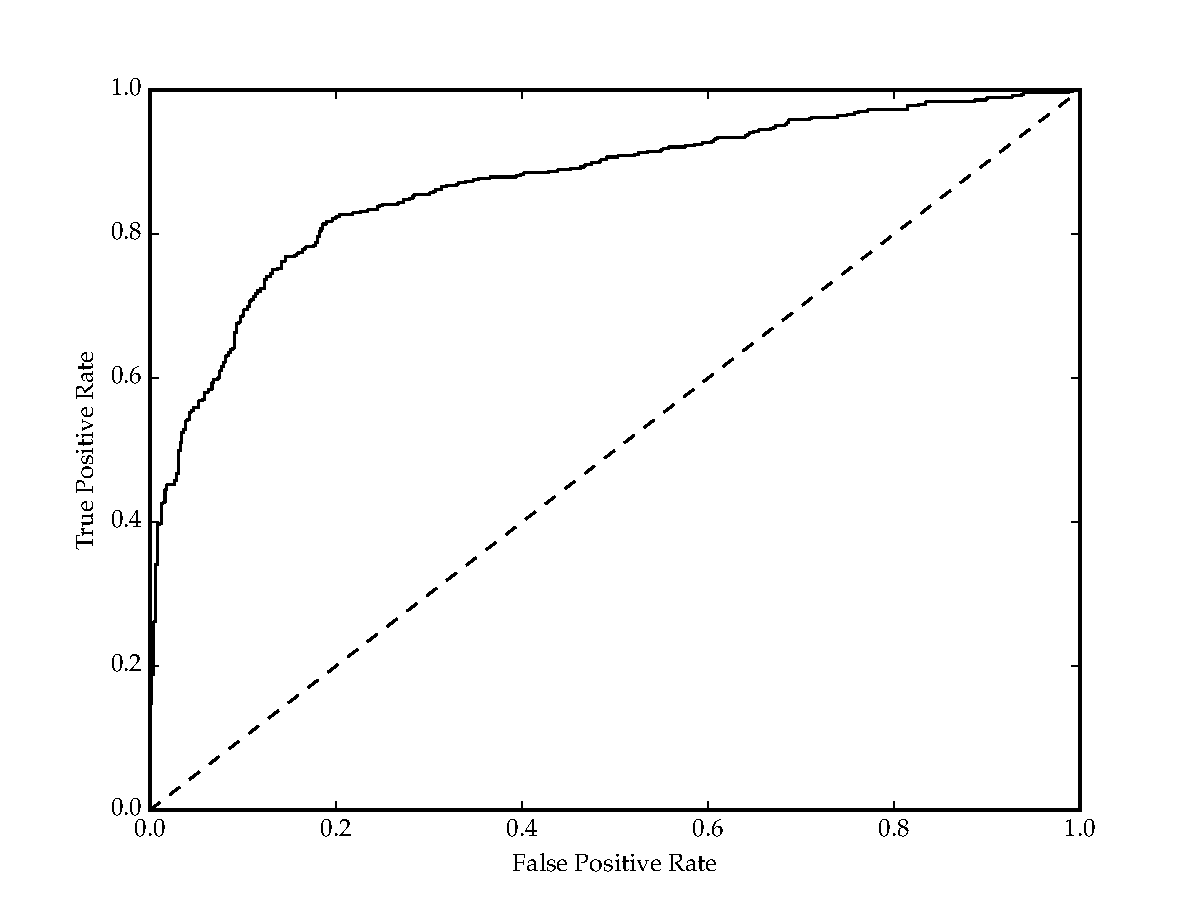
\includegraphics[width=.8\textwidth]{Figures/Chapter5/roc}
    \caption{An example of ROC curve. The dashed line is the ROC curve of a random classifier.}
    \label{fig:roc}
\end{figure}
To illustrate the behavior of the curve, it is useful to consider three extreme cases:
\begin{enumerate}
\item for a perfect classifier, which makes no errors, the curve goes from point $(0;0)$, to point $(1;0)$, to point $(1;1)$;
\item for a completely random classifier, which whatever the threshold always produces the same number of false positives and true positives, the curve created is the line segment bounded by the points $(0;0)$ and $\,(1;1)$;
\item no reasonable classifier is assumed to produce a ROC curve whose points are located under the $(0;0)$, $\,(1;1)$ segment.
\end{enumerate}
An AUROC value of 0.5 describes a completely random classifier (since it is equal to the area of the triangle described by the extreme case 2), while an AUROC of 1 describes a perfect classifier (since it is equal to the area of the square described by the extreme case 1). Good classifiers have an AUROC score generally equal or higher than 0.8. Besides being a metric independent of class proportions, the AUROC also offers a probabilistic interpretation of its value, since it is equals to the probability that the classifier will rank a randomly chosen positive example higher than a randomly chosen negative example. For an extensive survey of ROC curves, see for example \cite{fawcett2006roc}.

\section{Results}
Here, we present the results obtained on the two experiments, \textbf{E1} and \textbf{E2}. Subsequently, we present an analysis of the performances obtained by the model on two use cases: one on synthetic data, and one on a real-world pathway.

\subsection{Results on the E1 Experiment}
Table \ref{tab:e1-results} shows the average accuracy on the 5 test folds obtained by each of the examined architectures on the \textbf{E1} experiment. Even though these results are obtained on a dataset approximately 15\% the size of the original one (consisting of 7036 induced subgraphs), we can already make some interesting observations about the task and the models:
\begin{itemize}
    \item the task can be learned, as evidenced by the gap between the baseline and all the examined models, which is approximately 13\% on average. This result verifies our initial assumption that it is indeed possible to predict robustness using only pathway structure;
    \item the comparison between the various \glspl{gcl} highlights the fact that there is no clear winner between the three tested architectures, which obtain very similar results when assessed on the same experimental conditions (\ie all models with/withour edge handling capabilities);
    \item as expected, adding edge handling to the \glspl{gcl} is beneficial to improve performances. On average, the models obtain a 1.8\% improvement in accuracy when edge handling is used.
\end{itemize}


\begin{table}[h!]
    \renewcommand\arraystretch{1.1}
    \caption{Results of the 5-fold CV evaluation of different \gls{dgn} architectures on the \textbf{E1} experiment, as explained in Section \ref{sec:pathway-experiments}. The suffix \quotes{-vanilla} indicates that the corresponding graph convolutional layer does not handle different edge contributions.}\label{tab:e1-results}
    \centering
    \begin{tabular}{lc}
        \toprule
            \Thead{Model}&  \Thead{Test Accuracy}\\
        \midrule
            Baseline & $0.7322\pm0.0000$\\
        \midrule
            GCN-vanilla & $0.8573\pm0.0087$ \\
            GIN-vanilla & $0.8567\pm0.0137$\\
            WLGCN-vanilla & $0.8624\pm0.0088$\\
        \midrule
            GCN & $0.8692\pm0.0140$\\
            GIN & $0.8684\pm0.0078$\\
            WLGCN & $0.8687\pm0.0117$\\
        \bottomrule
    \end{tabular}

\end{table}

In a second experiment, we assess whether depth (intendended as number of \gls{dgn} layers) is a good inductive for this task.To do so, we perform a \posthoc study the validation scores, to see how they relate to number of \gls{dgn} layers. Specifically, for each model, and for each number of layers from 1 to 8, we compute the average validation score obtained by all hyper-parameters configurations with an identical number of layers. Note that, although validation accuracy is in general an over-estimate of the true accuracy, the relative difference in performance as the number of layers change stays proportional independently of which specific data is used. In other words, we are not interested in the score by itself, but rather to the trend (increase or decrease) in performance in relation to the number of \gls{dgn} layers. Figure \ref{fig:e1-layering} clearly shows that, in all cases, increasing the number of layers improves accuracy, up to a certain depth (around 4-5 layers on average) where performances start to plateau. This provides evidence that depth is a good inductive bias for \glspl{dgn} on this task, up to some extent.

\begin{figure}[h!]
    \centering
    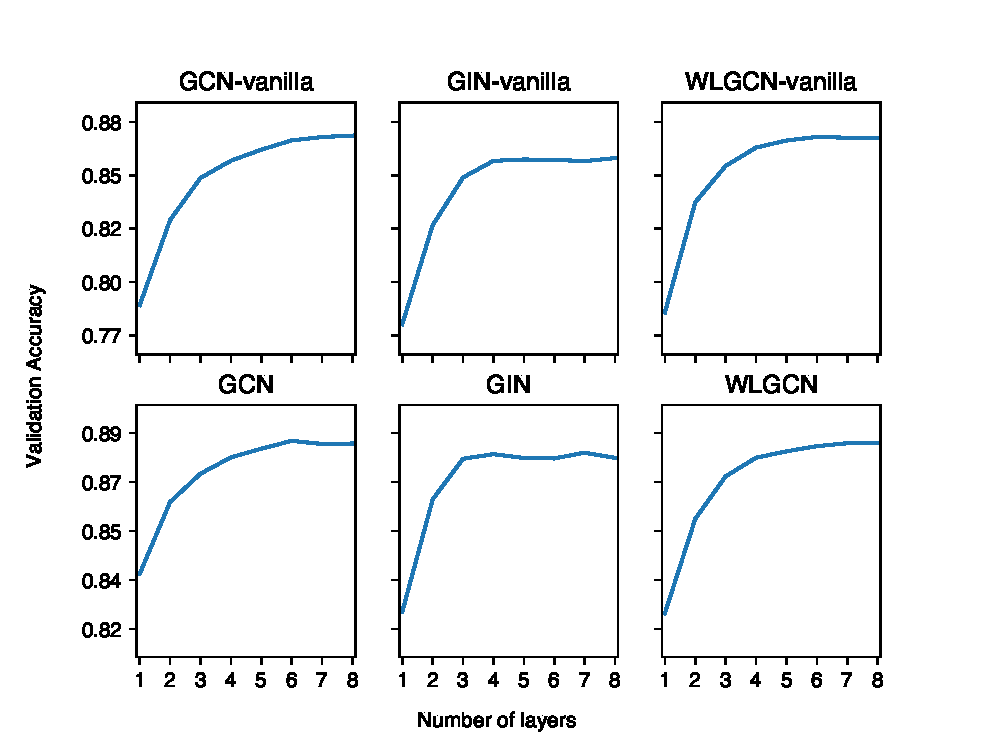
\includegraphics[width=.8\textwidth]{Figures/Chapter5/e1-layering}
    \caption{The effect of the number of \gls{dgn} layers to the performances of the models.}
    \label{fig:e1-layering}
\end{figure}

\subsection{Results on the E2 Experiments}\label{sec:e2-results}
For the second round of experiments, we fix the \gls{gcl} to the \gls{gcn} model with edge-handling capabilities, since it is the model that obtains the highest accuracy in \textbf{E1}.
The results of our experiments are reported in Table \ref{tab:e2-results}, where we average the computed metrics across the 5 test folds as usual.
\begin{table}[h!]
    \caption{Results of the 5-fold CV evaluation on various performance metrics. We report the global results (on the last row) as well as the results stratified by number of nodes per subgraph. For each stratification, we also report the related support (\ie the average number of graphs in the strata).}\label{tab:e2-results}
    \centering
    \footnotesize
    \renewcommand{\arraystretch}{1.2}
    \setlength{\tabcolsep}{0.7em}
    \begin{tabular}{lccccc}
      \toprule
      \Thead{Strata} & \Thead{Support} & \Thead{Accuracy} & \Thead{Sensitivity} & \Thead{Specificity} & \Thead{AUROC} \\
      \midrule
         1-10  & $243 (19)$ & $0.729 (0.020)$ & $0.851 (0.073)$ & $0.526 (0.113)$ & $0.820 (0.034)$\\
        11-20  & $711 (30)$ & $0.843 (0.006)$ & $0.919 (0.021)$ & $0.629 (0.050)$ & $0.892 (0.008)$\\
        21-30  & $526 (19)$ & $0.921 (0.008)$ & $0.969 (0.010)$ & $0.740 (0.052)$ & $0.954 (0.015)$\\
        31-40  & $967 (27)$ & $0.889 (0.012)$ & $0.937 (0.005)$ & $0.757 (0.040)$ & $0.950 (0.009)$\\
        41-50  & $1512 (21)$ & $0.928 (0.004)$ & $0.970 (0.008)$ & $0.635 (0.064)$ & $0.944 (0.011)$\\
        51-60  & $1679 (28)$ & $0.921 (0.004)$ & $0.971 (0.006)$ & $0.588 (0.038)$ & $0.950 (0.005)$\\
        61-70  & $1439 (23)$ & $0.947 (0.005)$ & $0.982 (0.006)$ & $0.644 (0.058)$ & $0.967 (0.005)$\\
        71-80  & $1159 (28)$ & $0.941 (0.006)$ & $0.980 (0.010)$ & $0.712 (0.087)$ & $0.972 (0.007)$\\
        81-90  & $372 (20)$ & $0.957 (0.008)$ & $0.998 (0.002)$ & $0.037 (0.075)$ & $0.925 (0.010)$\\
        91-100 & $378 (14)$ & $0.850 (0.017)$ & $0.964 (0.024)$ & $0.536 (0.061)$ & $0.888 (0.026)$\\
        \midrule
        \textbf{Overall} & $\mathbf{8985} (1)$ & $\mathbf{0.913} (0.003)$ & $\mathbf{0.965} (0.006)$ & $\mathbf{0.646} (0.042)$ & $\mathbf{0.948} (0.004)$\\
      \bottomrule
    \end{tabular}
\end{table}
In this case, we stratify the performances by number of nodes, in order to also analyze the model performances in relation to the size of the input subgraph. From the results, one can immediately see, by looking at the last row, how the model accurately predicts robustness better than all models tested in the \textbf{E1} phase by a large margin: this is probably caused by the largest size of the dataset, which usually results in major improvements with any \gls{ml} model, and in particular with \gls{dl} models. Specifically, we report an overall accuracy of $0.913 \pm 0.003$, as well as an AUROC of $0.948 \pm 0.004$. The model shows very high sensitivity ($0.965 \pm 0.006$) but a low specificity in comparison ($0.646 \pm 0.042$); this indicates that it is \quotes{harder} for the model to predict induced subgraphs that are not robust. This effect is a probable consequence of the class misproportion between negative and positive examples, which is around 86\% in favor of the positive class for this data sample. One result that is consistent across all measurements are the the very narrow standard deviations of the estimates, which indicate stable predictions regardless of the specific folds on which they are computed. To display this trend visually, we plot in Figure \ref{fig:e2-rolling-acc} the ROC curves obtained on the 5 test folds. Their similarity strongly indicates that the model performances are consistent across different test samples.
\begin{figure}
    \centering
    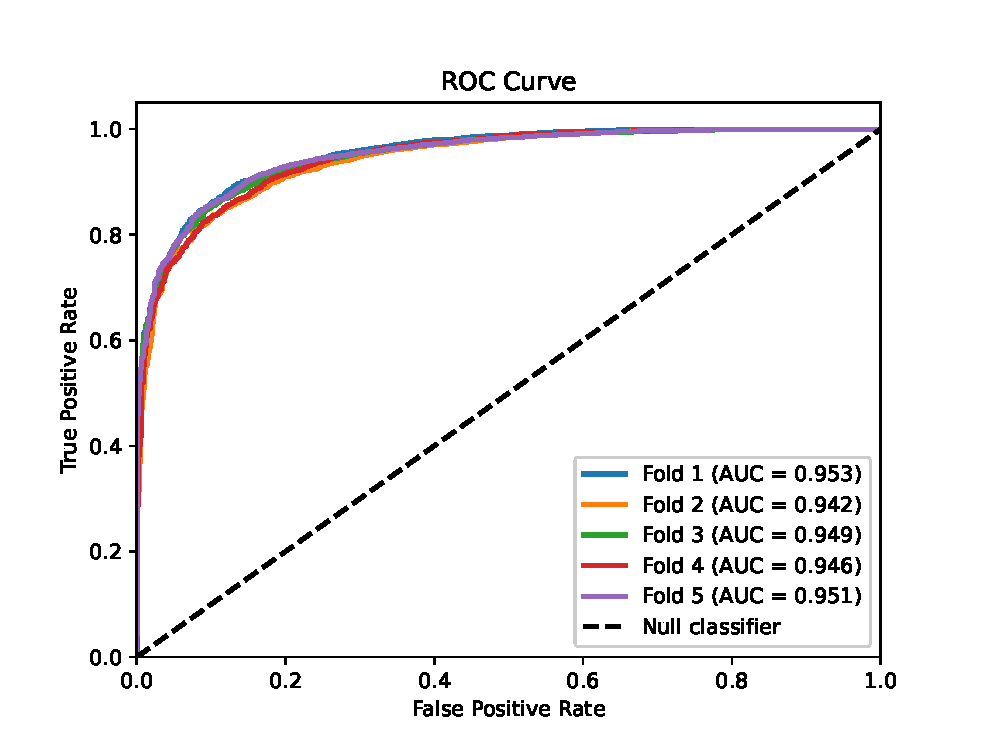
\includegraphics[width=.65\textwidth]{Figures/Chapter5/e2-roc-curve.eps}
    \caption{ROC curves for each of the five test folds. The black dashed line shows the performance of a baseline (\quotes{Null}) classifier that always predicts one class.}\label{fig:e2-roc-curve}
\end{figure}
The results of Table \ref{tab:e2-results} show a good performance of the model under the several stratifications tested. In particular, it performs better when dealing on subgraphs with 21-80 nodes, reaching an average in that strata AUROC of over 0.955. To better visualize this trend, we plot in Figure \ref{fig:e2-roc-curve} the rolling accuracy of the model, using a window size of 20, and averaging across the 5 test folds as usual. The plot clearly shows the improvement in accuracy as the number of nodes increases. Interestingly, when the size of the graph exceeds 80 nodes, the model performances start to decrease. This might be a consequence of the smaller sample sizes of subgraph with 81-100 nodes which occur in the dataset 3 times less on average than subgraphs with 21-80 nodes. The same trend can be noticed for smaller subgraphs, with up to 20 nodes. Finally, Figure \ref{fig:e2-conf-matrix} shows the confusion matrix of the predictions computed by the model, where the entries are the averages computed across the five test folds. In the plot, we can visualize the good performances of the model as regards the number of correctly predicted subgraphs (on the diagonal) with respect to the cases where the model makes wrong predictions. Looking at the anti-diagonal the confusion matrix, we can also see that the model has a higher rate of false positives than false negative. Again, this is expected behaviour due to class misproportion in the dataset.
\begin{figure}[h!]
    \begin{subfigure}[b]{0.48\linewidth}
    \centering
        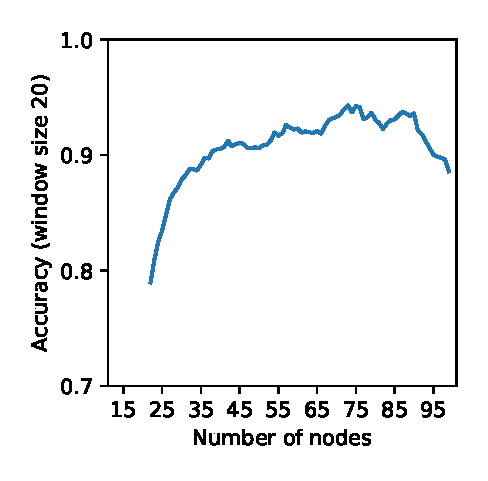
\includegraphics[height=130px]{Figures/Chapter5/e2-rolling-acc.eps}
        \subcaption{}\label{fig:e2-rolling-acc}
    \end{subfigure}
    %
    \begin{subfigure}[b]{0.48\linewidth}
        \centering
        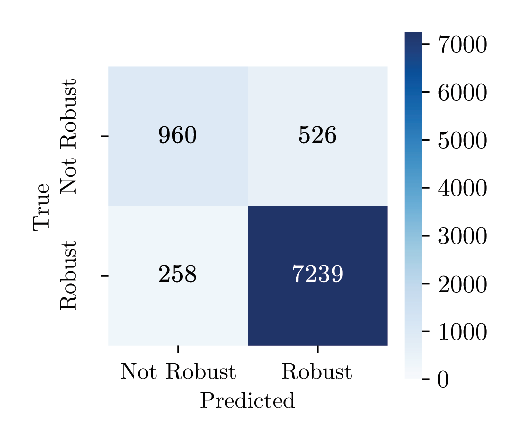
\includegraphics[height=130px]{Figures/Chapter5/e2-conf-matrix.eps}
        \subcaption{}\label{fig:e2-conf-matrix}
    \end{subfigure}
    \caption{({\scriptsize A}) Rolling mean accuracy (with a window of size 20), averaged over the 5 test folds, showing an increasing trend in performance as the number of graph nodes grows. ({\scriptsize B}) Confusion Matrix of the predictions computed by the model. Each entry of the matrix is the average of the corresponding entries in the five different confusion matrices of the test folds.}
\end{figure}

Lastly, we emphasize the fact that, once trained, the time needed to obtain a prediction from the model is in the order of milliseconds, while performing numerical simulations can be orders of magnitude slower. For this specific case, the simulation of most of the considered models (as detailed in Section \ref{sec:robustness-computation}) requires a amount of time in the order of minutes, while bigger models can take many hours to produce an output value. While training and evaluating the model is expensive, and can take hours, it needs to be performed only once. To conclude, we believe that, once perfected, methods inspired by our approach have the potential of enabling faster advances in understanding the functioning of cells through pathway modelling.

Following, we present two application cases of the model: the first is on the synthetic pathway shown in Figure \ref{fig:example-pathway}, and serves as an explanation tool of why the model performs sub-par in cases of smaller subgraphs; the second is an example of how the model can correctly infer the robustness relations in a real-world pathway.

\subsection{Application on Synthetic Data}
The lower prediction accuracy in the case of small graphs (1-10 nodes) can be put into perspective, in light of the fact the fact we trained the model with subgraphs in which kinetic, stoichiometric and initial concentration parameters have been omitted (as explained in Section \ref{sec:ppn}). In general, the smaller the graph, the higher the influence on its dynamics these parameters exert. As an example, let us consider the synthetic example of biochemical pathway introduced in Figure \ref{fig:example-pathway} and the corresponding pathway graph of Figure \ref{fig:pathway-graph}. Let us now consider the following kinetic and initial concentration (marking) parameters:
\begin{gather*}
  k1 = 1.0 \quad
  k3 = 0.01 \quad
  k5 = 0.01 \quad
  k7 = 0.3  \quad
  k2 = 5.0  \quad
  k4 = 0.1  \quad
  k6 = 5.0 \\
  m_0(A) = 50\quad
  m_0(B) = 50\quad
  m_0(C) = 100\quad
  m_0(D) = 100\\
  m_0(E) = 0\quad
  m_0(F) = 0\quad
  m_0(G) = 100\quad
  m_0(H) = 0.
\end{gather*}
We used these parameters to simulate the ODEs of Figure \ref{subfig:example-odes}, calculating the corresponding robustness by varying the initial concentration of each molecule in the interval $[-20\%,+20\%]$. The robustness values obtained with the simulations are displayed in Table \ref{tab:uc1-odes}. Analogously, in Table \ref{tab:uc1-predictions} we list the average and standard deviations obtained by the 5 different models evaluated in Section \ref{sec:e2-results} (one trained on the respective CV fold), when tasked to predict the robustness probabilities of some input/output pairs of interest.
\begin{table}[h!]
    % \scriptsize
    \centering
    \caption{({\scriptsize A}) Robustness values computed by numerical simulation of the ODEs in Figure \ref{fig:example-pathway}. Input molecules with initial concentration equal to 0 are omitted. Output molecules with identical robustness values are merged. ({\scriptsize B}) Probabilities of robustness obtained from the model for some relevant input/output combinations.}
    \begin{subtable}[b]{.59\linewidth}
      \centering
        \begin{tabular}{cccccc}
            \toprule
            \multirow{2}{*}{\textbf{Input}} & \multicolumn{5}{c}{\textbf{Output}}\\
             & \SF{A} & \SF{B} & \SF{C/D} & \SF{E/F} & \SF{G/H}\\
            \midrule
              \SF{A} & 1.00 & 0.73 & 0.99 & 1.00  & 1.00  \\
              \SF{B} & 1.00 & 0.73 & 0.99 & 1.00  & 1.00  \\
              \SF{C} & 1.00 & 1.00  & 0.00  & 0.99 & 0.99 \\
              \SF{D} & 1.00 & 1.00  & 0.00  & 0.99 & 0.99 \\
              \SF{G} & 1.00 & 1.00  & 1.00  & 1.00  & 0.50  \\
            \bottomrule
        \end{tabular}
        \caption{}\label{tab:uc1-odes}
    \end{subtable}%
    \begin{subtable}[b]{.39\linewidth}
        \centering
        \begin{tabular}{cc}
            \toprule
            \Thead{In/Out} & \Thead{Probability}\\
            \midrule
                $\SF{B}/\SF{A}$ & $0.3798 \pm 0.12$\\
                $\SF{A}/\SF{F}$ & $0.7254 \pm 0.18$\\
                $\SF{A}/\SF{H}$ & $0.8835 \pm 0.05$\\
                $\SF{C}/\SF{F}$ & $0.0793 \pm 0.11$\\
                $\SF{G}/\SF{H}$ & $0.2351 \pm 0.01$\\
            \bottomrule
        \end{tabular}
        \caption{}\label{tab:uc1-predictions}
    \end{subtable}
\end{table}
We remark that values in these two tables are not directly comparable: those in Table \ref{tab:uc1-odes} are exact robustness values, while those in Table \ref{tab:uc1-predictions} are probabilities of the robustness values to be greater than 0.5. In this specific case, the prediction turns out to be accurate in the case of input/output pairs corresponding to big induced subgraphs. This happens in the cases of the input/output pairs $A/F$ and $A/H$, whose induced subgraphs are among the largest ones. In contrast, the prediction is incorrect for $C/F$: in this case, the models predicts a small robustness probability, while the simulations give 0.99. We observe that the robustness value of this input/output combination is sensitive to the perturbation of parameters that have been discarded when constructing the dataset. In particular, if the initial (omitted) concentration of $C$ was $80$ instead of $100$, the robustness value of the pair $C/F$ would become $0.5$ rather than $0.99$. Another case when the model prediction is wrong is that of the pair The prediction turns out to be wrong also in the case of input $B/A$. In this case, the probability given by the network is under $0.50$, which contrasts to a value of $1$ obtained by the ODEs simulation. Even in this case, we notice that the parameters that have been omitted in the dataset might have a strong influence on the robustness, such as kinetic formulas and the multiplicity of the edge directed to node $B$. Finally, in the case of the pair $G/H$, the prediction gives a small probability of robustness and indeed the actual measured value is borderline ($0.50$). More in general, we observe that smaller subgraphs are less frequent than medium-sized subgraphs in the dataset. Thus, it is possible that the model has learned to be more accurate on the latter subgraphs (to maximize the accuracy), at the expense of making more errors when predicting the former.

\subsection{Application on a model of the EGF Pathway}
As a second use case, we consider the SBML model of the Epidermal Growth Factor (EGF) pathway proposed by Sivakumar et al. in \citep{sivakumar2011systems}. This model corresponds to model \texttt{BIOMD0000000394} of the BioModels database, and is shown in Figure \ref{fig:EGF} as represented by the CellDesigner tool \citep{funahashi2003celldesigner}. We adopt this visual representation style for this case study for readability, but the pathway can can be trivially translated into a \gls{ppn}.
\begin{figure}[t]
    \centering
    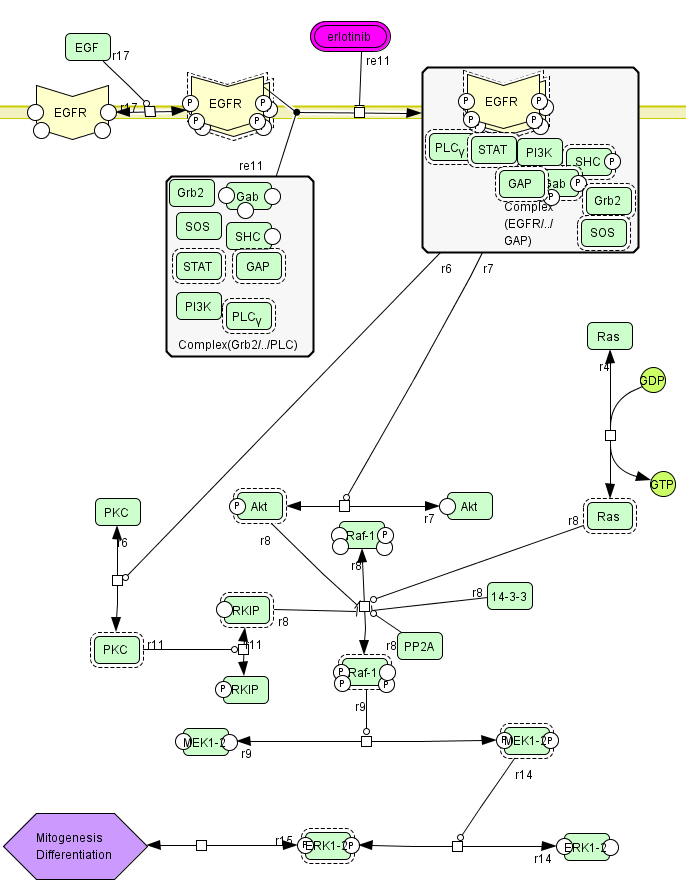
\includegraphics[width=12cm]{Figures/Chapter5/pathway394}
\caption{A model of the EGF pathway by Sivakumar et al. \citep{sivakumar2011systems}.Image generated form the SMBL file in the BioModels database using the CellDesigner tool.}\label{fig:EGF}
\end{figure}
The pathway describes, in a simplified way, the transduction of the EGF signal, and the consequent activation of the mitogenesis and cell differentiation processes (modelled as an abstract species in the pathway). When the EGF signal protein is available in the cell environment, it can be perceived by the receptor protein EGFR (where R stands for Receptor), which then initiates a cascade of reactions inside the cell, ultimately leading to the activation of mitogenesis and differentiation. The initial steps of the pathway give rise to a rather big complex, involving an activated EGFR dimer and a number of other proteins (the big box in the upper-left corner of Figure \ref{fig:EGF}). The formation of such complex is described in a very simplified way in this pathway model, by concentrating everything in only two reactions. The big complex then promotes a cascade of reactions inside the cell, which are modelled more in detail.

Considering the mitogenesis and differentiation (abstract) species as output (in pink, bottom left corner of Figure \ref{fig:EGF}), with respect to EGF and EGFR as input (in green and yellow, respectively, top left corner of Figure \ref{fig:EGF}), numerical simulations assign a very high robustness ($>0.995$) in both cases. This is actually expected in a signal transduction pathway, since it behaves as an amplifier that must be able to activate the target cell process despite of perturbations in the signal and receptor concentrations. On the other hand, if we look at the robustness of the first portion of the pathway up to the creation of the big complex, we can then observe a different behavior. Specifically, if we consider the big complex as output and EGF as input, we still obtain a very high robustness ($>0.999$). However, when the input is EGFR, we obtain a robustness value of only $0.19$. Again, this is not surprising, since EGF is modelled in the pathway as a promoter of the first reaction (\ie, it is not consumed), while EGFR is a reactant and it will be included in the big complex.

In this case, the model correctly captures the different roles of EGF and EGFR. Indeed, using EGF as input and the big complex as output, the model gives $0.9474 \pm 0.014$ as probability of robustness, whereas it gives $0.145 \pm 0.121$ when the input is with EGFR. The model captured also captures the robustness of the whole model, namely the previous case where either EGF or EGFR were considered as input, and the abstract mitogenesis and differentiation as output. Precisely, it gives probability $0.973 \pm 0.005$ with EGF as input and $0.970 \pm 0.008$ with EGFR as input.

\section{Conclusion and Further Work}
This work shows experimentally, and for the first time, that we can correlate structural properties of biological pathways to their dynamical properties. We consider this result very promising and deserving of further investigation. Indeed, the promise of this approach if that of creating a novel class of learning methods for pathways, which could help to better study the functioning of living cells.

We consider this approach impacting for two main reasons. Firstly, predicting dynamical properties of pathways with Deep Learning methods is faster than performing numerical or stochastic simulations. While the training process is expensive in terms of time required, it needs to be performed only once, and can be amortized nicely as more and larger subgraphs are used. Secondly, our approach works considering only a minimal amount of information regarding the pathway: its structure, an input and output node, and the types of nodes and relations between them. Hence, it is applicable even in cases where other information, such as kinetic constants, is not available.

One research direction to pursue in the immediate future concerns evaluating this architecture on datasets where the information we omitted in the present study has been added. For example, it would be interesting to assess how the addition of edge labels (multiplicities of reactants/products), or kinetic formulas, would affect performances. These additional information could be useful, for example, to help the preditions of the model in case of smaller subgraphs. Moreover, one could think to extend this approach to the assessment of other related dynamical properties of pathways, such as other notions of robustness, or even completely different ones such as monotonicity, or oscillatory and bistability properties.

We also believe this work opens up fascinating research scenarios to pursue in the medium term. One important aspect that needs further investigation is model explainability. Even though their predictive result are very often excellent, neural networks are sometimes seen as black-box since the exact function (in this case, from pathway structure to robustness) they approximate is difficult to characterize. One possible research direction is to investigate generative models, to uncover the underlying structure of pathway space and help design better predictive models, as well as provide better explanations to the decisions they take.
